\documentclass[11pt,a4paper]{article}
\usepackage[utf8]{inputenc}
\usepackage[english]{babel}
\usepackage{amsmath} % For mathematical symbols if any, good to have
\usepackage{amssymb} % For mathematical symbols if any, good to have
\usepackage{graphicx} % For images, if any
\usepackage{geometry}
\usepackage{titlesec}
\usepackage{enumitem}
\usepackage{array} % For more complex tables
\usepackage{tabularx} % For tables with fixed width columns
\usepackage{booktabs} % For professional quality tables
\usepackage{longtable} % For tables that span multiple pages
\usepackage{ragged2e} % For better justification (e.g., \RaggedRight)
\usepackage{parskip} % To have space between paragraphs instead of indent
\usepackage{hyperref} % For clickable links and cross-references
\usepackage{fancyhdr} % For custom headers and footers
\usepackage{lastpage} % To get the total number of pages for footer

\geometry{
    a4paper,
    left=2.5cm,
    right=2.5cm,
    top=2.5cm,
    bottom=2.5cm,
    headheight=15pt % Adjusted slightly based on fancyhdr recommendation
}

% Global settings for enumerated lists - more compact and professional
\setlist{nosep} % Removes extra vertical spacing

% Create consistent formatting for all enumeration and itemize environments with proper indentation
\setlist[enumerate,1]{leftmargin=2em, labelindent=0pt, itemsep=3pt}
\setlist[enumerate,2]{leftmargin=2.5em, labelindent=0pt, itemsep=2pt}
\setlist[enumerate,3]{leftmargin=3em, labelindent=0pt, itemsep=2pt}
\setlist[itemize,1]{leftmargin=2em, labelindent=0pt, label=\textbullet, itemsep=3pt}
\setlist[itemize,2]{leftmargin=2.5em, labelindent=0pt, label=\textendash, itemsep=2pt}
\setlist[itemize,3]{leftmargin=3em, labelindent=0pt, label=\textasteriskcentered, itemsep=2pt}

% Title formatting for sections and subsections - more compact and consistent
\titleformat{\section}
{\normalfont\bfseries}{\thesection.}{0.75em}{}
\titlespacing*{\section}{0pt}{1.25\baselineskip}{0.75\baselineskip}

\titleformat{\subsection}
{\normalfont\bfseries}{\thesubsection}{0.75em}{}
\titlespacing*{\subsection}{0pt}{0.75\baselineskip}{0.5\baselineskip}

\titleformat{\subsubsection}
{\normalfont\bfseries}{\thesubsubsection}{0.75em}{} % Changed from small to normal size for consistency
\titlespacing*{\subsubsection}{0pt}{0.5\baselineskip}{0.25\baselineskip}

% Consistent formatting for schedule headings
\newcommand{\scheduletitle}[1]{%
    \section*{#1}%
    \addcontentsline{toc}{section}{#1}%
}

\newcommand{\schedulesubtitle}[1]{%
    \subsection*{#1}%
}

\newcommand{\schedulesubsubtitle}[1]{%
    \subsubsection*{#1}%
}

% Hyperref setup for PDF metadata and links
\hypersetup{
    colorlinks=true,
    linkcolor=blue,       % Color for normal internal links
    citecolor=green,      % Color for bibliographical citations
    urlcolor=cyan,        % Color for external URLs
    pdftitle={Shareholders Agreement - The Augmented 4 Pty Ltd},
    pdfauthor={The Augmented 4 Pty Ltd and Shareholders},
    pdfsubject={Shareholders Agreement},
    pdfkeywords={Shareholders, Agreement, The Augmented 4, AI, Voice Agents}
}

% Page style with fancyhdr
\pagestyle{fancy}
\fancyhf{} % Clear all header and footer fields
\fancyhead[L]{\small Shareholders Agreement: The Augmented 4 Pty Ltd}
\fancyhead[R]{\small Effective Date: 12 june 2025}
\fancyfoot[C]{\small \thepage\ of \pageref{LastPage}}
\renewcommand{\headrulewidth}{0.4pt}
\renewcommand{\footrulewidth}{0.4pt}

% Small adjustments for more professional look
\setlength{\parindent}{0pt}
\setlength{\parskip}{6pt}

% Consistent table formatting
\newcommand{\standardtable}[1]{%
    \begin{tabular}{|p{4cm}|p{5cm}|p{6cm}|}
    \hline
    \textbf{IP Asset} & \textbf{Description} & \textbf{Details and Status} \\
    \hline
    #1
    \hline
    \end{tabular}
}

\begin{document}

\begin{titlepage}
    \centering
    \vspace*{1cm}
    
    % Company Logo
    
\includegraphics[width=0.4\textwidth]{/Users/domrutili/PROJECTS/Augmented-4-ShareHolder-Agreement/images/email.jpg}
    \vspace{0.5cm}
    
    {\normalsize\itshape removing friction between humans and AI}
    \vspace{1.5cm}
    
    {\LARGE\bfseries SHAREHOLDERS AGREEMENT}
    \vspace{1.5cm}
    
    {\Large relating to}
    \vspace{0.8cm}
    
    {\Large\bfseries THE AUGMENTED 4 PTY LTD}
    \vspace{0.4cm}
    
    {\normalsize (ACN 686 749 575)}
    \vspace{0.2cm}
    
    {\normalsize (ABN 20 686 749 575)}
    \vspace{3cm}
    
    \begin{flushright}
    \textbf{Dated: 12 june 2025}
    \end{flushright}
    \vspace{3cm}
    
    \rule{0.5\textwidth}{0.5pt}
    
    \vspace{0.5cm}
    {\small\itshape CONFIDENTIAL}
\end{titlepage}

\newpage
\tableofcontents
\newpage

% --- Main Clauses of the Agreement ---
\section{PARTIES}

\subsection{The Company}
\textbf{THE AUGMENTED 4 PTY LTD} (ACN 686 749 575), a proprietary company limited by shares incorporated in New South Wales, Australia pursuant to the Corporations Act 2001 (Cth), having its registered office at Unit 4, 5 Norman Avenue, Dolls Point, New South Wales 2219 (the \textbf{``Company''}).

\subsection{The Initial Shareholders}
\begin{enumerate}[label=(\arabic*)]
\item \textbf{DOMENICO RUTIGLIANO} of Unit 2, 5-7 Hercules Road, Brighton-le-Sands, New South Wales 2216, being the Founder and Chief Technology Officer (CTO) of the Company (hereinafter referred to as \textbf{``Shareholder A''});
\item \textbf{MICHAEL SCHEELHARDT} of [Insert Address], being the Founder and Chief Revenue Officer (CRO) of the Company (hereinafter referred to as \textbf{``Shareholder B''});
\end{enumerate}

(Shareholder A and Shareholder B are hereinafter collectively referred to as the \textbf{``Shareholders''} and individually as a \textbf{``Shareholder''}).  
\section{BACKGROUND}
\begin{enumerate}[label=\Alph*.]
\item The Company is incorporated under the Corporations Act 2001 and is governed by its Constitution and this Agreement.
\item The Shareholders are the legal and beneficial owners of the shares in the Company in the proportions set out in Schedule 1.
\item The Shareholders have agreed to regulate their relationship and the affairs of the Company in accordance with this Agreement.
\end{enumerate}

\section{RECITALS}
\begin{enumerate}[label=\Alph*.]
\item The Company is a proprietary company limited by shares, duly incorporated and existing under the laws of New South Wales, Australia, and is engaged in the Business (as defined herein).
\item The Initial Shareholders are the legal and beneficial owners of all the issued shares in the capital of the Company as at the date of this Agreement, in the proportions set out in Schedule 1.
\item The parties have agreed to enter into this Agreement to provide for the management and control of the Company and to regulate their respective rights, liabilities and obligations as Shareholders in the Company and in relation to the conduct of the Company's affairs, on the terms and conditions hereinafter set forth.
\item This Agreement records the terms upon which the Shareholders will govern their relationship inter se and with the Company, and it is intended to operate in conjunction with the Company's Constitution.
\end{enumerate}  % Formerly 2_background.tex
\section{INTERPRETATION}

\subsection{Definitions}
In this Agreement, unless the context otherwise requires:

``Acceding Shareholder'' means a person who becomes a party to this Agreement by executing a Deed of Accession;

``ACN'' means Australian Company Number;

``Agreement'' means this Shareholders Agreement, including all Schedules and any annexures, as amended from time to time in accordance with its terms;

``ASIC'' means the Australian Securities and Investments Commission;

``Associate'' has the meaning given to that term in section 12 of the Corporations Act;

``Auditor'' means the auditor of the Company appointed from time to time in accordance with this Agreement and the Corporations Act;

``Bad Leaver Event'' means a Bad Leaver Event as defined in the Leaver Provisions section of this Agreement;

``Board'' means the board of Directors of the Company as constituted from time to time;

``Business'' means the business of developing, designing, creating, marketing, selling, distributing, licensing, and supporting artificial intelligence (AI) powered voice agent solutions, related software, platforms, and services, and any other business carried on by the Company as may be determined by the Board and Shareholders from time to time in accordance with this Agreement;

``Business Day'' means a day (other than a Saturday, Sunday, or public holiday) on which banks are open for general banking business in Sydney, New South Wales, Australia;

``Cause'' or ``Founder Cause'' means, in relation to either Domenico Rutigliano or Michael Scheelhardt:
\begin{enumerate}[label=(\alph*)]
\item fraud or dishonesty;
\item gross misconduct;
\item material breach of this Agreement or their employment or engagement agreement with the Company, which has not been remedied within thirty (30) days of written notice;
\item conviction of an indictable offence;
\item serious breach of any statutory or common law duty owed to the Company;
\item conduct that is reasonably likely to bring the Company into serious disrepute;
\item persistent or serious breach of key obligations, including but not limited to:
    \begin{enumerate}[label=(\roman*)]
    \item making claims of personal ownership over Company assets (including IPR, customer relationships, or other proprietary information) contrary to the provisions of this Agreement;
    \item unauthorized disclosure of Company Confidential Information, IPR, customer data, or business strategies to third parties;
    \item attempting to misappropriate Company assets, including intellectual property, customer relationships, or business opportunities;
    \item taking actions that materially compromise or jeopardize the Company's ownership, development, commercialization, or market position;
    \item filing patents or other IP registrations in their own name or a third party's name based on Company-owned innovations;
    \item attempting to solicit Company clients or employees for a competing business venture.
    \end{enumerate}
\end{enumerate}

``CRO'' means the Chief Revenue Officer of the Company;

``Cessation Date'' means the date on which a Shareholder (or an Associate of a Shareholder, if applicable) ceases to be an employee or actively engaged service provider (including as a Director) of the Company or any of its subsidiaries for any reason;

``Change of Control'' means, in relation to the Company, an event where any person or group of associated persons (other than the existing Shareholders in their current proportions, or their Permitted Transferees) acquires, directly or indirectly, Control of the Company. 

``Control'' means either:
\begin{enumerate}[label=(\alph*)]
\item holding more than fifty percent (50\%) of the total voting rights attached to all issued Shares in the Company; or
\item having the ability to appoint or remove a majority of the Board members.
\end{enumerate}

For clarity:
\begin{enumerate}[label=(\roman*)]
\item the 50\% threshold refers to voting rights, not just share ownership;
\item indirect Control includes Control through one or more intermediaries;
\item existing Shareholders maintaining their current proportional holdings does not constitute a Change of Control;
\item transfers to Permitted Transferees (as defined in this Agreement) do not constitute a Change of Control.
\end{enumerate}

``Company'' means The Augmented 4 Pty Ltd (ACN 686 749 575);

``Confidential Information'' means all information (whether in oral, written, electronic, or any other form, and whether or not marked as confidential) disclosed by or on behalf of one party (the ``Disclosing Party'') to another party (the ``Receiving Party'') or otherwise coming to the knowledge of the Receiving Party, relating to the Disclosing Party, the Company, the Business, its customers, suppliers, finances, strategies, operations, products, services, technology (including Company IPR, AI models, algorithms, source code, and datasets), and the terms of this Agreement, which is not publicly known. It includes information known by a Shareholder by virtue of their involvement with the Company;

``Constitution'' means the constitution of the Company as adopted and amended from time to time;

``Continuing Shareholders'' means, in the context of a Right of First Refusal, the Shareholders other than the Selling Shareholder;

``Corporations Act'' means the Corporations Act 2001 (Cth) of Australia, as amended or replaced from time to time;

``CTO'' means the Chief Technology Officer of the Company, initially Domenico Rutigliano;

``Deadlock'' has the meaning given to it in the ``Exit Strategies and Deadlock Resolution'' section of this Agreement (sub-clause \ref{subsec:DeadlockResolution});

``Deed of Accession'' means a deed in the form set out in Annexure A (or such other form as approved by the Board) by which a new Shareholder agrees to be bound by this Agreement;

``Director'' means a director of the Company appointed from time to time;

``Drag-Along Notice'' means a notice given under the ``Drag-Along Rights'' sub-clause of this Agreement (sub-clause \ref{subsec:DragAlong});

``Effective Date'' means the date stated on the first page of this Agreement, being [9 June 2025];

``Exit Event'' means any of the events specified in the ``Exit Events'' sub-clause of this Agreement (sub-clause \ref{subsec:ExitEvents});

``Fair Market Value'' means the fair market value of a Share or other asset, determined in accordance with the valuation principles set out in this Agreement (particularly sub-clause \ref{subsec:CompanyValuationInternal}), or if not specified, as determined by an Independent Valuer acting as an expert;

``Financial Year'' means the period from 1 July in one year to 30 June in the next year, or such other period as the Board may determine in accordance with the Corporations Act;

``Independent Valuer'' means a reputable independent chartered accountant, accredited business valuer, or investment bank with at least ten (10) years of experience in valuing private technology companies (preferably in the AI sector), who is not the Auditor of the Company at the time of valuation (unless all parties to the valuation agree otherwise in writing), and who is appointed in accordance with the terms of this Agreement;

``Initial Shares'' means the 5,000,000 Ordinary Shares held by Domenico Rutigliano and the 5,000,000 Ordinary Shares held by Michael Scheelhardt as at the Effective Date, representing 42\% each of the total authorized share capital;

``Insolvency Event'' means, in relation to a party:
\begin{enumerate}[label=(\roman*)]
\item it is (or states that it is) an insolvent under administration or insolvent (each as defined in the Corporations Act);
\item it has a controller (as defined in the Corporations Act) appointed, or is in liquidation, in provisional liquidation, under administration or wound up or has had a receiver appointed to any part of its property;
\item it is subject to any arrangement, assignment, moratorium or composition, protected from creditors under any statute or dissolved (in each case, other than to carry out a reconstruction or amalgamation while solvent on terms approved by the other parties to this Agreement);
\item an application or order has been made (and in the case of an application, it is not stayed, withdrawn or dismissed within 30 days), resolution passed, proposal put forward, or any other action taken, in each case in connection with that person, which is preparatory to or could result in any of the things referred to in paragraphs (i), (ii) or (iii) above;
\item it is taken (under section 459F(1) of the Corporations Act) to have failed to comply with a statutory demand;
\item it is the subject of an event described in section 459C(2)(b) or section 585 of the Corporations Act (or it makes a statement from which another party to this Agreement reasonably deduces it is so subject); or
\item anything analogous to anything referred to above, or which has substantially similar effect, occurs with respect to it under the law of any applicable jurisdiction.
\end{enumerate}

``Intellectual Property Rights'' or ``IPR'' means all intellectual property rights and interests, whether registered or unregistered, conferred by statute, common law or equity in any part of the world, including but not limited to:
\begin{enumerate}[label=(\roman*)]
\item patents, utility models, rights in inventions, copyright (including future copyright and rights in the nature of or analogous to copyright), moral rights, database rights, rights in circuit layouts, designs, trademarks, service marks, business names, domain names, rights in get-up and trade dress;
\item rights in computer software (including source code, object code, algorithms, and APIs), AI models (including trained models, underlying architecture, and weights/parameters), datasets (including curated, processed, or annotated data used for training or operation of AI systems), and other forms of digital or electronic intellectual property;
\item rights in know-how, trade secrets, confidential information, and other proprietary information;
\item any application or right to apply for registration, renewal, or extension of any of these rights; and
\item all other intellectual property rights and equivalent or similar forms of protection existing anywhere in the world.
\end{enumerate}

``Key Executives'' means initially the CTO and the CRO, and any other person subsequently appointed by the Board to a senior executive role critical to the Company's operations or strategy;

``Key Performance Indicators'' or ``KPIs'' means the joint performance indicators and associated bonus structure detailed in Schedule 4, applicable to both the CTO and CRO;

``KPI Achievement Period'' means the period of twelve (12) months commencing on the Effective Date, as detailed in Schedule 4;

``KPI Schedule'' means Schedule 4 to this Agreement;

``Leaver'' means a Shareholder who experiences a Cessation Date;

``Lock-up Period'' means the period of five (5) years commencing on the Effective Date, or such other period as may be unanimously agreed in writing by all Shareholders;

``Majority Shareholders'' means, in the context of Drag-Along Rights, Shareholders holding the percentage of Shares specified in the ``Drag-Along Rights'' sub-clause (sub-clause \ref{subsec:DragAlong}) as being able to initiate a drag;

``New Active Customer'' has the meaning given in Schedule 4;

``Offered Shares'' means Shares offered for sale by a Selling Shareholder under a Right of First Refusal;

``Party'' means a party to this Agreement from time to time, including any person who accedes to this Agreement as a Shareholder or as the Company;

``Permitted Transferee'' means, in relation to a Shareholder:
\begin{enumerate}[label=(\roman*)]
\item if the Shareholder is an individual, their spouse, de facto partner, child, grandchild, parent, or sibling (or a trust established primarily for the benefit of one or more of such persons and/or the Shareholder, provided the Shareholder is a trustee and controls the voting rights of the Shares held by the trust);
\item a company wholly owned and controlled by that Shareholder (and/or by persons who are Permitted Transferees of that Shareholder under paragraph (i) above);
\item provided that, in each case, the proposed transferee executes a Deed of Accession prior to the registration of the Transfer and is not a competitor of the Company (as reasonably determined by the Board).
\end{enumerate}

``Proposed Transferee'' means a bona fide third party to whom a Selling Shareholder proposes to Transfer Shares, as identified in a Transfer Notice;

``Reserved Matters'' means the matters listed in Schedule 2 which require Requisite Shareholder Approval;

``Requisite Shareholder Approval'' means the approval of Shareholders holding at least the percentage of Shares specified in the Reserved Matters provisions of this Agreement, or where applicable, a higher percentage specified in Schedule 2 for a particular Reserved Matter;

``Rights Offer'' has the meaning given in the ``Future Funding and Capital Contributions'' sub-clause of this Agreement (sub-clause \ref{subsec:FutureFunding});

``Sale of the Company'' means a transaction or series of related transactions resulting in a Change of Control of the Company, or the sale, lease, or other disposal of all or substantially all of the assets of the Company;

``Schedule'' means a schedule to this Agreement;

``Selling Shareholder'' means a Shareholder proposing to Transfer Shares;

``Shares'' means fully paid ordinary shares in the capital of the Company. References to Shares include any shares of other classes that may be created and issued by the Company in the future, unless the context specifically refers to Ordinary Shares;

``Shareholder'' means any person registered as a holder of Shares in the Company's share register from time to time who is a party to this Agreement or has executed a Deed of Accession;

``Subscription Price'' means the price per New Share in a Rights Offer or other share issue, as defined in the ``Future Funding and Capital Contributions'' sub-clause (sub-clause \ref{subsec:FutureFunding});

``Tag-Along Notice'' means a notice given under the ``Tag-Along Rights'' sub-clause of this Agreement (sub-clause \ref{subsec:TagAlong});

``Transfer'' means, in relation to Shares, to sell, assign, transfer, convey, dispose of, grant an option over, declare a trust over, mortgage, charge, pledge, or otherwise encumber or create any security interest in or over, or permit any such action, whether directly or indirectly, voluntarily or involuntarily, or attempt or agree to do so;

``Transfer Notice'' means a notice given by a Selling Shareholder under the ``Right of First Refusal'' sub-clause of this Agreement (sub-clause \ref{subsec:ROFR}).

\subsection{Construction}
In this Agreement, unless the context otherwise requires:
\begin{enumerate}[label=(\alph*)]
\item headings and subheadings are for convenience only and do not affect the interpretation of this Agreement;
\item the singular includes the plural and vice versa;
\item a reference to any gender includes all genders;
\item a reference to a ``person'' includes any individual, firm, company, corporation, body corporate, government, state or agency of a state, trust or foundation, or any association, partnership or unincorporated body (whether or not having separate legal personality);
\item a reference to a party to this Agreement or any other document includes that party's successors, permitted assigns, and legal personal representatives;
\item a reference to this Agreement or any other document includes any variation, novation, replacement, or supplement of that document from time to time in accordance with its terms;
\item a reference to a clause, sub-clause, paragraph, Schedule, or annexure is to a clause, sub-clause, paragraph, Schedule, or annexure of or to this Agreement;
\item a reference to legislation or a provision of legislation includes any subordinate legislation made under it and any statutory instrument issued under it, and any modification, consolidation, re-enactment or replacement of any of them from time to time;
\item a reference to ``writing'' or ``written'' includes any method of representing or reproducing words, figures, or symbols in a visible and tangible form, including by email (but excluding SMS or other informal messaging systems unless expressly agreed for specific purposes);
\item a reference to ``AUD'', "\$'', or "dollars'' is a reference to Australian currency;
\item if a period of time is specified and dates from a given day or the day of an act or event, it is to be calculated exclusive of that day;
\item the words ``include'', ``includes'', and ``including'' are to be construed without limitation;
\item where a word or phrase is defined, its other grammatical forms have a corresponding meaning;
\item any timeframe or deadline that falls on a day that is not a Business Day shall be extended to the next Business Day;
\item a reference to "agreement'' includes any legally enforceable arrangement, understanding, or undertaking, whether or not in writing (unless the context requires it to be in writing).
\end{enumerate}

\subsection{Precedence}
In the event of any inconsistency between the provisions of the main body of this Agreement and any Schedule, the provisions of the main body of this Agreement shall prevail to the extent of the inconsistency, unless expressly stated otherwise in a Schedule for a specific purpose.


\section{SHAREHOLDINGS AND CAPITAL STRUCTURE}

\subsection{Fixed Shareholdings}
\begin{enumerate}[label=(\alph*)]
\item The parties acknowledge and agree that as at the Effective Date of this Agreement, the issued shares in the capital of the Company are held as follows:
    \begin{enumerate}[label=(\roman*)]
    \item Domenico Rutigliano: 5,000,000 Ordinary Shares, constituting 42\% of the total authorized shares.
    \item Michael Scheelhardt: 5,000,000 Ordinary Shares, constituting 42\% of the total authorized shares.
    \end{enumerate}
\item All shares held by both Shareholders are fully vested and beneficially owned by them without any vesting conditions or performance-based transfer obligations.
\item The parties acknowledge that this fixed shareholding structure replaces any previous arrangements regarding performance-based share transfers, with performance incentives now governed by the Joint Performance Bonus Structure detailed in Schedule 4.
\item The remaining 16\% of authorized shares are reserved for future investors (10\%) and employees/advisors (6\%) as detailed in the Future Funding section.
\end{enumerate}

\subsection{Future Share Issues by the Company}
\begin{enumerate}[label=(\alph*)]
\item The parties acknowledge that for any future capital raising, the Company may issue new shares. 
\item The issue of any new shares by the Company shall be subject to:
    \begin{enumerate}[label=(\roman*)]
    \item The pre-emptive rights and other provisions concerning share issues as set out in this Agreement and the Constitution;
    \item Equal opportunity for both Shareholders to maintain their proportional shareholding;
    \item Board approval by unanimous resolution;
    \item Compliance with all applicable laws and regulations.
    \end{enumerate}
\item Any new share issue shall result in the dilution of all then-current Shareholders proportionally to their respective shareholdings, unless otherwise agreed by unanimous resolution of the Shareholders.
\end{enumerate}

\subsection{Share Transfer Restrictions}
\begin{enumerate}[label=(\alph*)]
\item Neither Shareholder shall transfer, encumber, or otherwise dispose of any shares except in accordance with this Agreement and the Constitution.
\item Any proposed transfer of shares shall be subject to:
    \begin{enumerate}[label=(\roman*)]
    \item The Right of First Refusal provisions in this Agreement;
    \item Board approval by unanimous resolution;
    \item Maintenance of the intended equal shareholding structure where possible;
    \item Compliance with all applicable laws and regulations.
    \end{enumerate}
\end{enumerate}

\subsection{Investor Share Pool}
\begin{enumerate}[label=(\alph*)]
\item The Company shall maintain a designated pool of 1,190,476 Preference Shares (Non-Voting) (constituting 10\% of the total authorized share capital) reserved for future third-party external investors (the ``Investor Share Pool'').
\item These shares shall:
    \begin{enumerate}[label=(\roman*)]
    \item Be created as new shares by the Company;
    \item Not come from the personal holdings of either Shareholder;
    \item When issued, dilute both Shareholders proportionally;
    \item Be subject to the terms of investment as a Reserved Matter.
    \end{enumerate}
\item Upon issuance of shares from the Investor Share Pool:
    \begin{enumerate}[label=(\roman*)]
    \item The total issued share capital will increase accordingly;
    \item Both Shareholders will be diluted proportionally;
    \item The terms of such investment shall require approval as a Reserved Matter.
    \end{enumerate}
\end{enumerate}

\subsection{Investor Vesting and Transfer Restrictions}
\begin{enumerate}[label=(\alph*)]
\item \textbf{Vesting of Investor Shares:}
    \begin{enumerate}[label=(\roman*)]
    \item Shares issued to investors shall vest only upon full payment of the agreed investment amount.
    \item Partial payments shall create proportional vesting rights.
    \item The Board shall maintain a vesting register tracking investment payments and vesting status.
    \end{enumerate}

\item \textbf{Five-Year Lock-up Period:}
    \begin{enumerate}[label=(\roman*)]
    \item All shareholders (including investors) are subject to a mandatory five-year lock-up period from the date of share issuance.
    \item During this period, no transfer of shares is permitted except:
        \begin{enumerate}[label=(\alph*)]
        \item With unanimous Board approval;
        \item In case of a qualifying Exit Event;
        \item To Permitted Transferees (subject to Board approval).
        \end{enumerate}
    \end{enumerate}

\item \textbf{Share Transfer Payment Structure:}
    \begin{enumerate}[label=(\roman*)]
    \item Any approved share transfer payment shall be structured as installments based on:
        \begin{enumerate}[label=(\alph*)]
        \item The Company's available profits after accounting for:
            \begin{itemize}
            \item Research and Development requirements
            \item Working capital needs
            \item Growth and expansion plans
            \item Technology infrastructure investments
            \item Market conditions and opportunities
            \end{itemize}
        \item Maximum installment size limited to 25% of available profits per quarter
        \item Board's assessment of the Company's financial health
        \end{enumerate}
    \item The Board shall establish a Share Transfer Reserve Account to manage installment payments
    \end{enumerate}

\item \textbf{Board Assessment of Transfer Capacity:}
    \begin{enumerate}[label=(\roman*)]
    \item Prior to approving any share transfer, the Board must conduct a comprehensive assessment including:
        \begin{enumerate}[label=(\alph*)]
        \item Current and projected R\&D requirements
        \item Growth opportunities and capital needs
        \item Market conditions and competitive landscape
        \item Working capital requirements
        \item Technology infrastructure needs
        \item Impact on existing operations
        \end{enumerate}
    \item The Board must document its assessment and rationale
    \item Annual review of transfer capacity assessment criteria
    \end{enumerate}

\item \textbf{Protection of Company Operations:}
    \begin{enumerate}[label=(\roman*)]
    \item Share transfer payments must not:
        \begin{enumerate}[label=(\alph*)]
        \item Impair the Company's ability to fund R\&D
        \item Compromise working capital requirements
        \item Hinder growth opportunities
        \item Affect technology infrastructure investments
        \item Impact employee retention programs
        \end{enumerate}
    \item The Board may suspend or adjust installment payments if necessary to protect operations
    \end{enumerate}

\item \textbf{Transfer Process and Documentation:}
    \begin{enumerate}[label=(\roman*)]
    \item All transfer requests must be submitted in writing with:
        \begin{enumerate}[label=(\alph*)]
        \item Proposed transfer timing
        \item Requested payment schedule
        \item Impact assessment on company operations
        \item Proposed risk mitigation measures
        \end{enumerate}
    \item Board review within 30 business days
    \item Detailed documentation of decision rationale
    \end{enumerate}
\end{enumerate}

\textit{Note: The removal of performance-based share transfers is balanced by the comprehensive Joint Performance Bonus Structure in Schedule 4, which provides financial incentives for both Shareholders to achieve the Company's growth and quality targets.} 

\subsection{Share Structure Summary}

The following table provides a comprehensive overview of The Augmented 4 Pty Ltd's capital structure:

\begin{table}[H]
\centering
\begin{tabularx}{\textwidth}{|l|X|c|c|c|}
\hline
\textbf{Share Class} & \textbf{Holders \& Purpose} & \textbf{Authorized} & \textbf{Issued} & \textbf{\% of Total} \\
\hline
\multicolumn{5}{|c|}{\textbf{CURRENT ISSUED SHARES}} \\
\hline
Ordinary Shares (Voting) & Founders & 10,000,000 & 10,000,000 & 84.0\% \\
\hline
\multicolumn{5}{|c|}{\textbf{RESERVED SHARE POOLS}} \\
\hline
Preference Shares (Non-Voting) & Investors & 1,190,476 & 0 & 10.0\% \\
\hline
Employee Ordinary Shares & Employees & 714,286 & 0 & 6.0\% \\
(Non-Voting) & & & & \\
\hline
\multicolumn{5}{|c|}{\textbf{TOTALS}} \\
\hline
\textbf{Total Authorized} & \textbf{All Classes Combined} & \textbf{11,904,762} & \textbf{10,000,000} & \textbf{100.0\%} \\
\hline
\end{tabularx}
\caption{The Augmented 4 Pty Ltd - Capital Structure Overview}
\end{table}

\subsubsection{Key Structure Features}

\begin{enumerate}[label=(\alph*)]
\item \textbf{Founder Control}: Domenico and Michael maintain 100\% voting control through equal holdings of Ordinary Shares (Voting).

\item \textbf{Equal Partnership}: Both founders hold identical 42\% stakes with equal voting rights (50\% each of voting shares).

\item \textbf{Investor Protection}: 10\% reserved for investors through Preference Shares with liquidation preference and anti-dilution rights.

\item \textbf{Employee Participation}: 6\% reserved for employee equity participation without diluting founder voting control.

\item \textbf{Scalable Structure}: Reserved pools allow growth without immediate dilution of founder positions.

\item \textbf{Governance Clarity}: Three distinct share classes with clearly defined rights and restrictions.
\end{enumerate} 
\section{INTELLECTUAL PROPERTY AND CONFIDENTIALITY}

\subsection{Current IP Ownership}
\begin{enumerate}[label=(\alph*)]
\item All Intellectual Property Rights related to The Augmented 4 Pty Ltd's technology, including but not limited to AI voice agent technologies, algorithms, source code, models, and associated intellectual property (the ``Company IP'') are currently owned exclusively by Domenico Rutigliano.

\item The Company acknowledges and agrees that Domenico Rutigliano is the sole and exclusive owner of all Company IP as of the date of this Agreement.

\item The Company and other Shareholders acknowledge that this ownership arrangement is integral to the Company's initial structure and valuation.

\item This IP ownership structure is separate from and does not affect the share class structure or voting rights under this Agreement.
\end{enumerate}

\subsection{Future IP Assignment}
\begin{enumerate}[label=(\alph*)]
\item Upon the occurrence of a Capital Raise Event (as defined below), Domenico Rutigliano agrees to assign all Company IP to The Augmented 4 Pty Ltd.

\item For the purposes of this section, a ``Capital Raise Event'' means any:
    \begin{enumerate}[label=(\roman*)]
    \item equity investment into the Company by a third party from the Preference Share pool of at least AUD 750,000 in a single transaction or series of related transactions within a 12-month period;
    \item initial public offering of the Company's shares; or
    \item other capital raising event of at least AUD 750,000 as unanimously agreed by the Ordinary Shareholders (Voting).
    \end{enumerate}

\item In consideration for the assignment of Company IP, the Company shall pay to Domenico Rutigliano:
    \begin{enumerate}[label=(\roman*)]
    \item a one-time payment of AUD 100,000; and
    \item any applicable taxes associated with the assignment.
    \end{enumerate}

\item \textbf{Personal Loan Repayment Obligation:} Upon receipt of the AUD 100,000 IP compensation payment, Domenico Rutigliano shall immediately repay in full all personal loans provided by Michael Scheelhardt to Domenico Rutigliano as documented in Schedule 6 (Personal Loan Register) to this Agreement. The parties acknowledge that these personal loans are separate from and independent of this Shareholders Agreement, but the repayment obligation is incorporated herein for commercial certainty and enforceability.

\item Alternative Revenue-Based Compensation:
    \begin{enumerate}[label=(\roman*)]
    \item If the Capital Raise Event does not generate sufficient funds to pay the AUD 100,000 compensation, the Company shall pay Domenico Rutigliano through a revenue-sharing arrangement.
    \item The percentage of revenue to be allocated shall be determined by unanimous Board approval (requiring both founders' consent).
    \item This revenue-sharing arrangement shall continue until the full AUD 100,000 compensation has been paid.
    \item Upon reaching the total compensation of AUD 100,000, Domenico Rutigliano shall execute the IP Assignment Deed.
    \item The Board shall review and adjust the revenue-sharing percentage quarterly to ensure both Company sustainability and timely compensation, subject to unanimous founder approval.
    \item \textbf{Personal Loan Repayment under Revenue-Sharing:} If IP compensation is paid through revenue-sharing, Domenico Rutigliano shall repay all personal loans from Michael Scheelhardt (as documented in Schedule 6) through monthly interest-free installments. The monthly repayment amount shall be proportional to the monthly IP compensation received, ensuring full repayment is completed simultaneously with the completion of the AUD 100,000 IP compensation payment.
    \end{enumerate}

\item The assignment shall be documented in a formal IP Assignment Deed, which shall:
    \begin{enumerate}[label=(\roman*)]
    \item be executed within 30 days of either:
        \begin{enumerate}[label=(a)]
        \item the Capital Raise Event; or
        \item the completion of the AUD 100,000 payment through revenue sharing;
        \end{enumerate}
    \item include comprehensive schedules of all assigned IP;
    \item contain customary warranties and indemnities; and
    \item be in a form reasonably satisfactory to both founders.
    \end{enumerate}

\item IP assignment decisions require unanimous approval of Ordinary Shareholders (Voting) as a Reserved Matter.
\end{enumerate}

\subsection{Interim IP License}
\begin{enumerate}[label=(\alph*)]
\item Until the occurrence of a Capital Raise Event, Domenico Rutigliano grants to the Company an exclusive, worldwide, royalty-free license to use, modify, and commercialize the Company IP for the purposes of conducting the Business.

\item This license shall:
    \begin{enumerate}[label=(\roman*)]
    \item be irrevocable except in the case of material breach by the Company;
    \item include the right to sublicense with unanimous Board approval (both founders' consent);
    \item terminate automatically upon the assignment of Company IP to the Company; and
    \item survive the termination of this Agreement until the IP assignment occurs.
    \end{enumerate}

\item Sublicensing rights and material IP licensing decisions require unanimous approval of Ordinary Shareholders (Voting).
\end{enumerate}

\subsection{Technology Protection and Governance}
\begin{enumerate}[label=(\alph*)]
\item The Company shall maintain:
    \begin{enumerate}[label=(\roman*)]
    \item Comprehensive IP registration and protection strategy;
    \item Regular IP audits and reviews;
    \item Secure source code repositories;
    \item AI model version control and security;
    \item Data protection and privacy compliance systems;
    \item Technical documentation of all IP assets.
    \end{enumerate}

\item All material IP protection decisions require unanimous Board approval.

\item IP strategy and protection measures shall be reported to all Ordinary Shareholders (Voting) quarterly.

\item Preference Shareholders (Non-Voting) receive information rights regarding IP protection but no decision-making authority.

\item Employee Ordinary Shareholders (Non-Voting) have no IP governance rights but benefit from IP value through their economic participation.
\end{enumerate}

\subsection{Employee IP Contributions}
\begin{enumerate}[label=(\alph*)]
\item All IP created by employees in the course of their employment automatically belongs to the Company upon IP assignment completion.

\item Prior to IP assignment, employee IP contributions are licensed to the Company under the same terms as the interim license.

\item Employee IP assignment agreements shall include:
    \begin{enumerate}[label=(\roman*)]
    \item Assignment of all work-related IP to the Company;
    \item Moral rights waivers where applicable;
    \item Confidentiality and non-disclosure obligations;
    \item Post-employment IP restrictions.
    \end{enumerate}

\item Employee IP contributions do not affect their Employee Ordinary Share (Non-Voting) allocations or vesting schedules.
\end{enumerate}

\subsection{Confidentiality Obligations by Share Class}
\begin{enumerate}[label=(\alph*)]
\item \textbf{All Shareholders} must maintain strict confidentiality of:
    \begin{enumerate}[label=(\roman*)]
    \item All Company IP and technical information;
    \item Business strategies and commercial information;
    \item Customer data and relationships;
    \item Financial information and performance data;
    \item This Agreement and its terms.
    \end{enumerate}

\item \textbf{Ordinary Shareholders (Voting)} have access to all confidential information necessary for governance decisions.

\item \textbf{Preference Shareholders (Non-Voting)} receive confidential information subject to their information rights and investment protection needs.

\item \textbf{Employee Ordinary Shareholders (Non-Voting)} receive confidential information necessary for their employment duties and share participation.

\item Confidentiality obligations:
    \begin{enumerate}[label=(\roman*)]
    \item Survive termination of this Agreement indefinitely;
    \item Apply to all representatives and advisors;
    \item Include return/destruction of confidential materials upon request;
    \item Require immediate reporting of unauthorized disclosures.
    \end{enumerate}

\item Breach of confidentiality may result in forfeiture of unvested Employee Ordinary Shares (Non-Voting) and other remedies available at law or equity.
\end{enumerate}

\subsection{Tax Treatment and Compliance}
\begin{enumerate}[label=(\alph*)]
\item \textbf{Tax Treatment Disclaimer:} Each party acknowledges that the Company does not provide tax advice, and the parties shall obtain their own independent tax advice regarding the IP compensation and related transactions. Nothing in this Agreement shall be construed as a representation or warranty regarding the tax treatment of any payment, assignment, or transfer. All taxes (including income tax, GST, or capital gains tax, if any) arising from or in connection with the IP compensation shall be the sole responsibility of the recipient, unless otherwise agreed in writing.
\end{enumerate} % IP and Confidentiality provisions
\section{LEAVER PROVISIONS}

\subsection{Application and Definitions}
\begin{enumerate}[label=(\alph*)]
\item The provisions of this section apply equally to both Founder Shareholders:
    \begin{enumerate}[label=(\roman*)]
    \item Domenico Rutigliano (Chief Technology Officer); and
    \item Michael Scheelhardt (Chief Revenue Officer).
    \end{enumerate}
\item For the purposes of this section, the following definitions apply:
    \begin{enumerate}[label=(\roman*)]
    \item \textbf{``Founder''} means either Domenico Rutigliano or Michael Scheelhardt, as applicable;
    \item \textbf{``Other Founder''} means the Founder who is not the subject of the leaver provisions;
    \item \textbf{``Protected Period''} means the period of four (4) years commencing on the Effective Date;
    \item \textbf{``Cessation Date''} means the date on which a Founder's employment or engagement with the Company ceases.
    \end{enumerate}
\end{enumerate}

\subsection{Good Leaver and Bad Leaver Definitions}
\begin{enumerate}[label=(\alph*)]
\item \textbf{``Cause''} means, in relation to the termination of a Founder's employment or engagement:
    \begin{enumerate}[label=(\roman*)]
    \item fraud or dishonesty;
    \item gross misconduct;
    \item material breach of this Agreement or employment agreement, not remedied within sixty (60) days of written notice;
    \item conviction of an indictable offence;
    \item serious breach of statutory or common law duty owed to the Company;
    \item conduct reasonably likely to bring the Company into serious disrepute;
    \item persistent breach of confidentiality or IP obligations.
    \end{enumerate}

\item \textbf{``Good Reason''} means any of the following occurring without the Founder's consent:
    \begin{enumerate}[label=(\roman*)]
    \item material reduction in duties, responsibilities, or authority;
    \item material breach by the Company of this Agreement or employment agreement;
    \item material failure to provide agreed resources for business development;
    \item compulsory relocation of principal workplace by more than 50 kilometers.
    \end{enumerate}

\item \textbf{``Good Leaver Event''} means cessation due to:
    \begin{enumerate}[label=(\roman*)]
    \item death;
    \item permanent incapacity preventing performance of duties for three (3) continuous months;
    \item termination by the Company other than for Cause;
    \item resignation for Good Reason.
    \end{enumerate}

\item \textbf{``Bad Leaver Event''} means cessation due to:
    \begin{enumerate}[label=(\roman*)]
    \item voluntary resignation without Good Reason during the Protected Period;
    \item termination by the Company for Cause;
    \item material breach of post-termination obligations.
    \end{enumerate}
\end{enumerate}

\subsection{Consequences of Good Leaver Event}
\begin{enumerate}[label=(\alph*)]
\item If a Founder's cessation constitutes a Good Leaver Event:
    \begin{enumerate}[label=(\roman*)]
    \item The Founder retains all Shares held at the Cessation Date;
    \item All rights and transfer restrictions continue to apply;
    \item The Founder maintains all shareholder rights under this Agreement.
    \end{enumerate}
\end{enumerate}

\subsection{Mandatory Mediation Before Bad Leaver Penalties}
\begin{enumerate}[label=(\alph*)]
\item Before any Bad Leaver penalties are applied, the parties must engage in mandatory mediation:
    \begin{enumerate}[label=(\roman*)]
    \item \textbf{Mediation Notice:} The Company must provide 30 days written notice of intention to apply Bad Leaver penalties
    \item \textbf{Mediation Process:} Independent mediator appointed within 10 Business Days from list of commercial mediators
    \item \textbf{Good Faith Participation:} All parties must participate in good faith for up to 20 Business Days
    \item \textbf{Scope:} Mediation covers dispute resolution, alternative arrangements, and penalty mitigation
    \item \textbf{Costs:} Mediation costs shared equally between Company and departing Founder
    \item \textbf{Confidentiality:} All mediation discussions remain confidential and without prejudice
    \end{enumerate}
\item Bad Leaver penalties may only be applied if mediation fails to resolve the matter within the specified timeframe.
\end{enumerate}

\subsection{Consequences of Bad Leaver Event}
\begin{enumerate}[label=(\alph*)]
\item If a Founder's cessation constitutes a Bad Leaver Event occurring within the Protected Period and mediation has been unsuccessful:
    \begin{enumerate}[label=(\roman*)]
    \item \textbf{Graduated Share Reduction:} The Founder must offer for sale a portion of Shares (``Bad Leaver Shares'') to the Company or Other Founder:
        \begin{enumerate}[label=(\alph*)]
        \item Year 1: 20\% of total shareholding;
        \item Year 2: 15\% of total shareholding;
        \item Year 3: 10\% of total shareholding;
        \item Year 4: 5\% of total shareholding.
        \end{enumerate}
    \item \textbf{Serious Misconduct Adjustment:} For fraud, dishonesty, gross misconduct, or serious IP breach, an additional 5\% (maximum 25\% total in any circumstance).
    \item \textbf{Absolute Penalty Cap:} Under no circumstances shall Bad Leaver penalties exceed 25\% of total shareholding, regardless of the nature or timing of the Bad Leaver Event.
    \end{enumerate}

\item \textbf{Purchase Price:}
    \begin{enumerate}[label=(\roman*)]
    \item Fraud/dishonesty/gross misconduct/serious IP breach: 70\% of Fair Market Value;
    \item Voluntary resignation without Good Reason: 85\% of Fair Market Value;
    \item Other Bad Leaver Events: Fair Market Value.
    \end{enumerate}

\item \textbf{Valuation Process:}
    \begin{enumerate}[label=(\roman*)]
    \item Independent Valuer appointed within 30 Business Days;
    \item Valuation report within 20 Business Days;
    \item Costs shared equally between Company and departing Founder;
    \item \textbf{Appeal Mechanism:} Either party may request second independent valuation within 10 Business Days if they dispute the initial valuation by more than 20\%;
    \item \textbf{Final Valuation:} If second valuation requested, final value is the average of both valuations;
    \item \textbf{Appeal Costs:} Party requesting second valuation pays for it unless the difference exceeds 25\%, in which case costs are shared equally.
    \end{enumerate}

\item \textbf{Purchase Option:}
    \begin{enumerate}[label=(\roman*)]
    \item Other Founder has first right to purchase Bad Leaver Shares;
    \item If declined, Company may purchase;
    \item 30 Business Days to exercise option after valuation;
    \item Purchase price paid in cash at completion.
    \end{enumerate}
\end{enumerate}

\subsection{Board Position and Governance Rights}
\begin{enumerate}[label=(\alph*)]
\item Upon any Founder's Cessation Date:
    \begin{enumerate}[label=(\roman*)]
    \item Immediate resignation from Director position;
    \item Board appoints successor with appropriate expertise;
    \item Director appointment rights suspended:
        \begin{enumerate}[label=(\alph*)]
        \item Good Leaver: 6 months;
        \item Bad Leaver: 24 months or until holding less than 25\% of shares.
        \end{enumerate}
    \end{enumerate}

\item During suspension of governance rights:
    \begin{enumerate}[label=(\roman*)]
    \item Reserved Matters require 75\% shareholder approval;
    \item Other Founder maintains full governance rights.
    \end{enumerate}

\item \textbf{Permanent Suspension:} For serious misconduct (fraud, criminal conviction, IP misappropriation), the Board may permanently suspend governance rights by unanimous resolution.
\end{enumerate}

\subsection{Transition Obligations}
\begin{enumerate}[label=(\alph*)]
\item Upon Cessation Date, departing Founder must:
    \begin{enumerate}[label=(\roman*)]
    \item Provide comprehensive documentation of responsibilities;
    \item Transfer all access credentials and administrative rights;
    \item Participate in knowledge transfer for up to 30 days;
    \item Return all Company property and confidential information;
    \item Certify compliance with transition requirements.
    \end{enumerate}

\item Company may withhold 25\% of payments until satisfactory completion of transition obligations.
\end{enumerate}

\subsection{Reputation Protection}
\begin{enumerate}[label=(\alph*)]
\item If a former Founder engages in conduct causing material reputational harm, specifically including:
    \begin{enumerate}[label=(\roman*)]
    \item \textbf{False Public Statements:} Knowingly false or misleading public statements about the Company's technology, financial position, or business practices made through media, social media, or industry forums;
    \item \textbf{Criminal Conviction:} Conviction of a criminal offence involving dishonesty, fraud, or conduct directly related to technology or business operations;
    \item \textbf{Industry Disrepute:} Conduct that results in formal sanctions, censure, or exclusion by relevant professional bodies or industry associations;
    \item \textbf{Customer/Partner Interference:} Deliberately undermining Company relationships by making false statements to customers, partners, or suppliers about the Company's capabilities or reliability;
    \item \textbf{Regulatory Violations:} Conduct resulting in regulatory action against the former Founder that directly impacts the Company's reputation or business operations.
    \end{enumerate}

\item \textbf{Materiality Threshold:} Reputational harm must be material, meaning it demonstrably affects the Company's business relationships, revenue, or ability to operate effectively.

\item \textbf{Notice and Cure Period:} Company must provide 30 days written notice specifying the conduct and allowing opportunity to remedy where possible.

\item \textbf{Limited Remedy:} Company may require sale of up to 15\% of remaining shares at Fair Market Value, subject to the valuation appeal mechanism.

\item \textbf{Exclusions:} This clause does not apply to legitimate business competition, honest criticism, or good faith disputes about Company matters.
\end{enumerate}

\subsection{Equal Treatment Principle}
\begin{enumerate}[label=(\alph*)]
\item All provisions in this section apply equally to both Founders regardless of their specific roles or responsibilities.
\item No Founder receives preferential treatment in leaver provisions.
\item Both Founders have identical rights and obligations under these provisions.
\end{enumerate}  % Formerly Leaver_Provisions.tex
\section{Transfer of Shares}

\subsection{General Prohibition and Share Class Transfer Restrictions}
\begin{enumerate}[label=(\alph*)]
\item No Shareholder may Transfer any Shares, whether directly or indirectly, except as expressly permitted by this Agreement and subject to the specific restrictions applicable to each share class.
\item \textbf{Ordinary Shares (Voting) - Founder Lock-up:} During the Lock-up Period (being a period of five (3) years from the Effective Date), holders of Ordinary Shares (Voting) shall not Transfer any such Shares except:
    \begin{enumerate}[label=(\roman*)]
    \item with the prior unanimous written consent of all Ordinary Shareholders (Voting);
    \item pursuant to the provisions of the Exit Events clause of this Agreement;
    \item to a Permitted Transferee in accordance with subsection \ref{subsec:PermittedTransfers} below.
    \end{enumerate}
\item \textbf{Preference Shares (Non-Voting) - Investor Transfers:} Preference Shares (Non-Voting) may be transferred subject to:
    \begin{enumerate}[label=(\roman*)]
    \item Right of first refusal to Ordinary Shareholders (Voting);
    \item Board approval (unanimous founder consent);
    \item Transferee execution of Deed of Accession;
    \item Compliance with tag-along and drag-along provisions.
    \end{enumerate}
\item \textbf{Employee Ordinary Shares (Non-Voting) - Employment Restrictions:} Employee Ordinary Shares (Non-Voting) are subject to:
    \begin{enumerate}[label=(\roman*)]
    \item Vesting schedules and forfeiture provisions;
    \item Company right of first refusal;
    \item Transfer restrictions during employment and for 12 months post-termination;
    \item Board approval for any transfers.
    \end{enumerate}
\item Any purported Transfer of Shares not made in strict accordance with this Agreement shall be void and of no effect, and the Company shall not recognise or register any such Transfer.
\end{enumerate}

\subsection{Permitted Transfers by Share Class} \label{subsec:PermittedTransfers}
\begin{enumerate}[label=(\alph*)]
\item \textbf{Ordinary Shares (Voting):} Founders may transfer to Permitted Transferees including:
    \begin{enumerate}[label=(\roman*)]
    \item Immediate family members;
    \item Family trusts where founder is beneficiary;
    \item Wholly-owned corporate entities;
    \item Transfers pursuant to estate planning or succession.
    \end{enumerate}
\item \textbf{Preference Shares (Non-Voting):} Investors may transfer to:
    \begin{enumerate}[label=(\roman*)]
    \item Affiliated investment funds or entities;
    \item Other institutional investors approved by Board;
    \item Transfers pursuant to fund liquidation or succession.
    \end{enumerate}
\item \textbf{Employee Ordinary Shares (Non-Voting):} Employees may transfer only:
    \begin{enumerate}[label=(\roman*)]
    \item Vested shares to immediate family members;
    \item Pursuant to estate planning with Company approval;
    \item Back to Company under buyback provisions.
    \end{enumerate}
\item No Transfer to a Permitted Transferee shall be effective until the Permitted Transferee has executed a Deed of Accession in accordance with subsection \ref{subsec:DeedOfAccession}.
\end{enumerate}

\subsection{Right of First Refusal by Share Class} \label{subsec:ROFR}
\begin{enumerate}[label=(\alph*)]
\item \textbf{Ordinary Shares (Voting) ROFR:} Any proposed transfer of Ordinary Shares (Voting) must first be offered to:
    \begin{enumerate}[label=(\roman*)]
    \item The other Ordinary Shareholder (Voting) with full right of first refusal;
    \item If declined, to the Company for buyback;
    \item If declined, subject to Board approval for third-party transfer.
    \end{enumerate}
\item \textbf{Preference Shares (Non-Voting) ROFR:} Any proposed transfer must be offered to:
    \begin{enumerate}[label=(\roman*)]
    \item Other Preference Shareholders pro-rata to their holdings;
    \item Ordinary Shareholders (Voting) if declined by Preference Shareholders;
    \item Third parties with Board approval if declined by all shareholders.
    \end{enumerate}
\item \textbf{Employee Ordinary Shares (Non-Voting) ROFR:} Any proposed transfer must be offered to:
    \begin{enumerate}[label=(\roman*)]
    \item The Company at fair market value;
    \item Other employees participating in the share plan;
    \item Ordinary Shareholders (Voting) if declined by Company and employees.
    \end{enumerate}
\item ROFR procedures require 30 Business Days notice and acceptance period.
\item Valuation for ROFR purposes shall be determined by independent valuation or Board-approved methodology.
\end{enumerate}

\subsection{Tag-Along Rights by Share Class} \label{subsec:TagAlong}
\begin{enumerate}[label=(\alph*)]
\item \textbf{Founder Share Transfers:} If Ordinary Shareholders (Voting) propose to transfer shares representing 25\% or more of voting control, all other shareholders have tag-along rights:
    \begin{enumerate}[label=(\roman*)]
    \item Other Ordinary Shareholders (Voting): Full pro-rata tag-along rights;
    \item Preference Shareholders (Non-Voting): Tag-along rights based on liquidation preference;
    \item Employee Ordinary Shareholders (Non-Voting): Tag-along rights for vested shares only.
    \end{enumerate}
\item \textbf{Investor Share Transfers:} If Preference Shareholders propose to transfer 50\% or more of their holdings:
    \begin{enumerate}[label=(\roman*)]
    \item Other Preference Shareholders have pro-rata tag-along rights;
    \item Ordinary Shareholders (Voting) have tag-along rights at their discretion;
    \item Employee Ordinary Shareholders have no tag-along rights.
    \end{enumerate}
\item Tag-along procedures require 30 Business Days notice and 20 Business Days exercise period.
\item All tag-along participants receive same price per share adjusted for share class rights.
\end{enumerate}

\subsection{Drag-Along Rights} \label{subsec:DragAlong}
\begin{enumerate}[label=(\alph*)]
\item \textbf{Founder Drag-Along Authority:} Ordinary Shareholders (Voting) holding 75\% or more of voting shares may exercise drag-along rights over all other shareholders.
\item \textbf{Enhanced Protections for Non-Voting Shareholders:}
    \begin{enumerate}[label=(\roman*)]
    \item Independent valuation required confirming fair market value;
    \item Preference Shareholders receive liquidation preference protection;
    \item Employee Ordinary Shareholders receive acceleration of vesting for unvested shares;
    \item All shareholders receive same economic treatment adjusted for share class rights.
    \end{enumerate}
\item \textbf{Board Approval Requirement:} Drag-along requires unanimous Board approval (both founders) confirming:
    \begin{enumerate}[label=(\roman*)]
    \item Transaction is in Company's best interests;
    \item Fair value provided to all shareholders;
    \item Proper protection for minority shareholders.
    \end{enumerate}
\item \textbf{Legal and Regulatory Compliance:}
    \begin{enumerate}[label=(\roman*)]
    \item The Drag-Along Sale must comply with all applicable laws, including the Corporations Act 2001 (Cth).
    \item Shareholders must receive all necessary disclosures and documentation.
    \item The transaction must not prejudice minority shareholders unfairly.
    \end{enumerate}
\item \textbf{Minimum Protection Period:} No drag-along may be exercised within 36 months of Effective Date except with unanimous shareholder consent.
\item Drag-along procedures require 30 Business Days notice and independent fairness opinion.
\item \textbf{Valuation Floor:}
    \begin{enumerate}[label=(\roman*)]
    \item The offer must meet a minimum valuation threshold agreed by the Board.
    \end{enumerate}
\end{enumerate}

\subsection{Employee Share Forfeiture and Buyback}
\begin{enumerate}[label=(\alph*)]
\item \textbf{Unvested Share Forfeiture:} Upon termination of employment:
    \begin{enumerate}[label=(\roman*)]
    \item All unvested Employee Ordinary Shares (Non-Voting) are forfeited to Company;
    \item Forfeiture occurs automatically without compensation;
    \item Good leaver vs. bad leaver provisions apply per employment agreements.
    \end{enumerate}
\item \textbf{Vested Share Buyback:} Company has option to repurchase vested Employee Ordinary Shares:
    \begin{enumerate}[label=(\roman*)]
    \item At fair market value determined by independent valuation;
    \item Exercise period of 90 days post-termination;
    \item Payment terms of 30 days cash or 12-month installments;
    \item Employee may retain shares if Company declines buyback option.
        \end{enumerate}
\item \textbf{Acceleration Provisions:} Vesting acceleration occurs upon:
    \begin{enumerate}[label=(\roman*)]
    \item Change of control (drag-along or sale of Company);
    \item Involuntary termination without cause;
    \item Death or permanent disability;
    \item Board-approved acceleration for retention purposes.
    \end{enumerate}
\end{enumerate}

\subsection{Deed of Accession by Share Class} \label{subsec:DeedOfAccession}
\begin{enumerate}[label=(\alph*)]
\item Any person acquiring Shares (whether by transfer from an existing Shareholder or by subscription for new Shares) must execute a Deed of Accession in the form set out in Annexure A before being registered as a Shareholder.
\item The Deed of Accession ensures that all new Shareholders are bound by the terms of this Agreement.
\item No Share transfer or new Share issue shall be registered until the relevant Deed of Accession has been executed.
\end{enumerate}

\subsection{Valuation Methodology for Transfers}
\begin{enumerate}[label=(\alph*)]
\item \textbf{Independent Valuation Required for:}
    \begin{enumerate}[label=(\roman*)]
    \item All drag-along transactions;
    \item Employee share buybacks;
    \item Disputes over ROFR pricing;
    \item Third-party transfers requiring Board approval.
    \end{enumerate}
\item \textbf{Valuation Methodology:}
    \begin{enumerate}[label=(\roman*)]
    \item Discounted cash flow analysis;
    \item Comparable company multiples;
    \item Recent transaction pricing;
    \item Asset-based valuation where appropriate.
    \end{enumerate}
\item \textbf{Share Class Adjustments:}
    \begin{enumerate}[label=(\roman*)]
    \item Preference Shares valued including liquidation preference;
    \item Employee Ordinary Shares valued on as-converted basis;
    \item Voting premium applied to Ordinary Shares (Voting) where appropriate.
    \end{enumerate}
\item Valuation costs borne by party requesting transfer unless otherwise specified.
\end{enumerate}

\subsection{No Encumbrances by Share Class}
\begin{enumerate}[label=(\alph*)]
\item \textbf{Ordinary Shares (Voting):} No encumbrances without unanimous founder consent.
\item \textbf{Preference Shares (Non-Voting):} Limited encumbrances permitted for:
    \begin{enumerate}[label=(\roman*)]
    \item Fund financing arrangements with Board approval;
    \item Institutional investor portfolio financing;
    \item Security interests approved by Board.
    \end{enumerate}
\item \textbf{Employee Ordinary Shares (Non-Voting):} No encumbrances permitted except:
    \begin{enumerate}[label=(\roman*)]
    \item Company security interests for loan arrangements;
    \item Court-ordered attachments;
    \item Tax liens with Company notification.
\end{enumerate}
\end{enumerate}

\subsection{Company's Obligation to Register Transfers}
\begin{enumerate}[label=(\alph*)]
\item Company shall register transfers complying with this Agreement and Constitution.
\item Board may refuse registration of non-compliant transfers.
\item Share class-specific transfer requirements must be satisfied.
\item Proper Deed of Accession required for all transfers.
\item Transfer register shall maintain separate records for each share class.
\end{enumerate}
% Add LaTeX labels to subsections for \ref{} if needed, e.g., \label{sec:transfer_of_shares}  % Enhanced version of original 5_share_transfer.tex
\section{EXIT MECHANISMS}

\subsection{Exit Events} \label{subsec:ExitEvents}
The following constitute Exit Events:
\begin{enumerate}[label=(\alph*)]
\item Initial Public Offering (IPO);
\item Trade sale of all or substantially all Company shares or assets;
\item Merger or consolidation resulting in change of control;
\item Winding up of the Company.
\end{enumerate}

\subsection{IPO Provisions}
\begin{enumerate}[label=(\alph*)]
\item Decision to pursue IPO requires 75\% Shareholder approval.
\item All Shareholders must cooperate with IPO process including:
    \begin{enumerate}[label=(\roman*)]
    \item accepting reasonable escrow arrangements;
    \item providing all required information;
    \item executing necessary documentation;
    \item appointing recommended advisers for technology and IP due diligence.
    \end{enumerate}
\end{enumerate}

\subsection{Trade Sale}
\begin{enumerate}[label=(\alph*)]
\item Board may recommend trade sale to Shareholders.
\item Sale requires 75\% Shareholder approval.
\item Process must ensure:
    \begin{enumerate}[label=(\roman*)]
    \item competitive tension;
    \item protection of Company IP, particularly AI models and voice technology;
    \item fair value for Shareholders;
    \item appropriate warranties and indemnities related to technology performance.
    \end{enumerate}
\end{enumerate}

\subsection{Buy-Out Mechanism}
\begin{enumerate}[label=(\alph*)]
\item Any Shareholder may offer to buy all other Shareholders' Shares.
\item Offer must be:
    \begin{enumerate}[label=(\roman*)]
    \item in writing;
    \item at fair market value determined by an independent valuer with expertise in technology companies;
    \item on identical terms to all Shareholders;
    \item fully funded or subject to reasonable funding conditions.
    \end{enumerate}
\item Other Shareholders have 30 Business Days to make a counter-offer or accept.
\end{enumerate}

\subsection{Deadlock Provisions} \label{subsec:DeadlockResolution}
\begin{enumerate}[label=(\alph*)]
\item A ``Deadlock'' shall be deemed to exist if:
    \begin{enumerate}[label=(\roman*)]
    \item a resolution on a Reserved Matter requiring unanimous approval has been voted upon at two consecutive properly convened Board meetings or Shareholder meetings at least 14 days apart;
    \item the resolution has not been passed due to dissenting votes or abstentions of one or more Directors or Shareholders; and
    \item in the reasonable opinion of at least one Director or Shareholder, such failure to pass the resolution is materially detrimental to the Company's business.
    \end{enumerate}
\item If a Deadlock arises and cannot be resolved within 30 Business Days through good faith negotiations between the Shareholders, any Shareholder may serve a written notice (a ``Deadlock Notice'') on the other Shareholders and the Company, identifying the nature of the Deadlock.
\item \textbf{Cooling-Off Period and Structured Negotiation:} Upon receipt of a Deadlock Notice:
    \begin{enumerate}[label=(\roman*)]
    \item A mandatory cooling-off period of 20 Business Days shall commence (the ``Cooling-Off Period'').
    \item During the Cooling-Off Period, the Shareholders shall refrain from taking any material action related to the subject matter of the Deadlock that could exacerbate the situation or prejudice any party's position.
    \item Within 5 Business Days following the Deadlock Notice, the Shareholders shall meet to discuss the Deadlock in person or by video conference with the objective of understanding each party's position and concerns in detail.
    \item The Shareholders shall use this meeting to identify possible compromise solutions and establish common ground, documented in a shared memorandum.
    \item The Shareholders shall each designate a senior representative who has not been directly involved in the disputed matter (where possible) to lead follow-up discussions.
    \item These designated representatives shall meet at least twice during the Cooling-Off Period to explore compromise solutions.
    \end{enumerate}
\item \textbf{Structured Mediation Process:} If the Deadlock remains unresolved after the Cooling-Off Period:
    \begin{enumerate}[label=(\roman*)]
    \item The Shareholders shall jointly appoint an independent, qualified mediator with experience in commercial disputes in the technology sector from a list of pre-approved mediators maintained by the Australian Disputes Centre or a similar organization (the ``Mediator'').
    \item If the Shareholders cannot agree on a Mediator within 5 Business Days, each Shareholder shall nominate one mediator, and those nominees shall together select the Mediator within a further 5 Business Days.
    \item The mediation shall commence within 15 Business Days of the Mediator's appointment and follow a structured process including:
        \begin{itemize}
        \item Pre-mediation submissions to be provided to the Mediator at least 5 Business Days before the mediation;
        \item A joint opening session to set the agenda and process;
        \item Both joint and separate caucus sessions at the Mediator's discretion;
        \item Focused discussions on resolving the specific issue(s) causing the Deadlock; and
        \item Documented proposed solutions from each party.
        \end{itemize}
    \item The mediation shall continue for a period of up to 20 Business Days, unless extended by mutual agreement of the Shareholders.
    \item The costs of the mediation shall be borne equally by the Shareholders, regardless of the outcome.
    \item All discussions in the mediation shall be confidential and without prejudice.
    \end{enumerate}
    \item \textbf{Enhanced Mediation Commitment:} The Shareholders agree that:
    \begin{enumerate}[label=(\roman*)]
        \item They will participate in the mediation in good faith with a genuine commitment to explore compromises and solutions;
        \item Each Shareholder shall be represented in the mediation by a person with full authority to make binding decisions (or with immediate access to such authority);
        \item If the Mediator believes that additional sessions would be productive, the mediation period shall be extended for up to 10 additional Business Days;
        \item If the Mediator proposes a compromise solution that they believe is fair and reasonable, the Shareholders commit to seriously consider such proposal before rejecting it;
        \item If the Mediator determines that a particular Shareholder is not participating in good faith, they may document this in a report to be considered in any subsequent proceedings.
        \end{enumerate}
    \item \textbf{Third-Party Expert Facilitation:} If the mediation has not resolved the Deadlock:
    \begin{enumerate}[label=(\roman*)]
    \item Before proceeding to the Fair Valuation Buyout Option or Texas Shootout procedure, the Shareholders shall consider appointing an independent industry expert with relevant technical or commercial expertise.
    \item The expert shall provide a non-binding evaluation of the disputed matter, meet with the Board and key executives to understand the technical, commercial, or operational aspects of the dispute, prepare a written recommendation for resolving the Deadlock, and present recommendations at a special Board meeting.
        \item The appointment of such expert shall be by mutual agreement of the Shareholders, and the costs shall be borne equally.
        \item The process shall be completed within 30 Business Days of the expert's appointment.
        \item If no agreement is reached on appointing an expert, or if the expert's recommendation is not accepted by all Shareholders within 10 Business Days, then the Shareholders may proceed to the Fair Valuation Buyout Option.
        \end{enumerate}
\item \textbf{Fair Valuation Buyout Option:} If the Deadlock remains unresolved following the structured mediation process:
    \begin{enumerate}[label=(\roman*)]
    \item Before proceeding to the Texas Shootout procedure, any Shareholder (the ``Offering Shareholder'') may deliver a written notice (the ``Fair Value Buyout Notice'') offering to purchase all (but not less than all) of the Shares held by the other Shareholders (the ``Offeree Shareholders'').
    \item Upon delivery of a Fair Value Buyout Notice, an Independent Valuer shall be appointed to determine the Fair Market Value of the Shares.
    \item The Independent Valuer shall determine the Fair Market Value having regard to standard valuation methodologies appropriate for technology companies, the specific nature of the Company's AI voice agent business, historical financial performance and future projections, the value of intellectual property and technology, customer relationships and contracts, and market conditions.
    \item The Offeree Shareholders shall have 15 Business Days from receipt of the valuation report to accept or decline the offer.
    \item If declined, the Offeree Shareholders may deliver a counter Fair Value Buyout Notice within 10 Business Days.
    \end{enumerate}
\item \textbf{Texas Shootout Procedure:} If the Deadlock is not resolved through previous procedures, any Shareholder (the ``Initiating Shareholder'') may trigger the Texas Shootout procedure:
    \begin{enumerate}[label=(\roman*)]
    \item The Initiating Shareholder shall deliver a notice (the ``Shootout Notice'') to the other Shareholders offering either to purchase all their Shares or sell all the Initiating Shareholder's Shares at a specified price per Share.
    \item The Shootout Notice must specify the proposed price per Share, applicable payment terms, and completion date.
    \item The Recipient Shareholders shall have 20 Business Days to elect to either purchase all of the Initiating Shareholder's Shares or sell all of their Shares at the specified price.
    \item If the Recipient Shareholders fail to respond within the Response Period, they shall be deemed to have elected to sell all of their Shares to the Initiating Shareholder.
    \item Following the election, the purchasing Shareholder(s) shall be obligated to purchase, and the selling Shareholder(s) shall be obligated to sell, the relevant Shares at the specified price.
    \item If the purchasing Shareholder(s) fail to complete the purchase, the selling Shareholder(s) may either enforce the sale through legal proceedings or purchase the Shares of the defaulting Shareholder(s) at ninety percent (90\%) of the original price as a penalty.
    \end{enumerate}
\item As an alternative to the Texas Shootout procedure, the Shareholders may unanimously agree in writing to:
    \begin{enumerate}[label=(\roman*)]
    \item sell the entire Company to a third party;
    \item appoint an independent expert with casting vote authority on the specific matter causing the Deadlock; or
    \item implement any other agreed resolution mechanism.
    \end{enumerate}
\item The valuation of Shares for any transfer pursuant to this clause shall be the price specified in the Shootout Notice, unless the Shareholders unanimously agree to appoint an Independent Valuer to determine the Fair Market Value.
\item All parties shall cooperate fully with the procedures set out in this clause and shall execute all documents and take all actions necessary to give effect to any transfer of Shares resulting from these procedures.
\end{enumerate}  % This was named Exit Strategies & Deadlock Resolution in our discussions
\section{MANAGEMENT AND GOVERNANCE}

\subsection{Board Composition}
\begin{enumerate}[label=(\alph*)]
\item The Board shall consist of two (2) directors initially comprising:
    \begin{enumerate}[label=(\roman*)]
    \item Domenico Rutigliano as Chief Technology Officer (CTO)
    \item Michael Scheelhardt as Chief Revenue Officer (CRO)
    \end{enumerate}
\item Each Shareholder has the right to appoint and maintain one director on the Board.
\item The removal of any director requires the approval of the appointing Shareholder.
\item Any vacancy on the Board shall be filled by the Shareholder entitled to make the appointment.
\end{enumerate}

\subsection{Board Meetings}
\begin{enumerate}[label=(\alph*)]
\item Board meetings shall be held at least quarterly, and more frequently as required for the effective management of the Business.
\item Notice period for meetings shall be at least 7 Business Days, unless waived by all directors.
\item Quorum requires presence (in person or by electronic means) of all directors.
\item Meetings may be held by telephone, video conference or other electronic means agreed by the directors.
\item Written resolutions signed by all directors are as valid as resolutions passed at a meeting.
\end{enumerate}

\subsection{Management Roles and Responsibilities}
\begin{enumerate}[label=(\alph*), wide, labelwidth=!, labelindent=0pt]
\item The day-to-day management of the Company's business shall be conducted by the key executives appointed by the Board, subject to the overall direction and supervision of the Board and the budget and business plan approved by the Board and, where applicable, the Shareholders.
\item The initial key executives and their primary areas of responsibility are:

\subsubsection*{Chief Technology Officer (CTO) - Initially Domenico Rutigliano}
    \begin{itemize}
    \item Overall technical strategy, vision, and direction of the Company.
    \item Leading the development, implementation, and maintenance of the Company's AI voice agent technology, algorithms, software, and platforms.
    \item Overseeing the technical infrastructure, including its scalability, performance, and security, and managing the Company's data assets.
    \item Driving research and development (R\&D) initiatives to ensure the Company maintains technological leadership and fosters innovation.
    \item Managing and developing the Company's Intellectual Property portfolio related to its technology, in conjunction with any IP policies set by the Board.
    \item Leading, mentoring, and developing the technical team, fostering a culture of engineering excellence, collaboration, and continuous improvement.
    \item Identifying, assessing, and managing technology-related risks and ensuring compliance with relevant technical standards, best practices, and regulations.
    \item Reporting to the Board on all material technological matters.
    \end{itemize}

\subsubsection*{Chief Revenue Officer (CRO) - Initially Michael Scheelhardt}
    \begin{itemize}
    \item Developing and executing the Company's overall commercial strategy, go-to-market plans, and business development initiatives.
    \item Leading all sales, marketing, customer acquisition, and customer success efforts.
    \item Building and maintaining strong, long-term relationships with key customers, strategic partners, and other industry stakeholders.
    \item Identifying, evaluating, and pursuing new market opportunities, strategic partnerships, and channels for growth.
    \item Driving revenue growth, managing commercial operations, including developing pricing strategies, and leading contract negotiations.
    \item Developing and managing the Company's brand identity, market positioning, and all related communications.
    \item Providing market intelligence, customer feedback, and competitive analysis to the Board and technical teams to inform product development and overall business strategy.
    \item Reporting to the Board on all material commercial matters.
    \end{itemize}
\item The specific duties and responsibilities of any executive officer may be further defined, varied, or supplemented by the Board from time to time. The Board may also appoint other officers (such as a Chief Executive Officer, Chief Financial Officer, etc.) as it deems necessary, and the appointment of such officers may be a Reserved Matter.
\end{enumerate}

\subsection{Growth Commitment and Resource Allocation}
\begin{enumerate}[label=(\alph*), wide, labelwidth=!, labelindent=0pt]
\item \textbf{Customer Growth Target:} The Shareholders hereby commit to supporting the growth of the Company's customer base to at least 1,000 active customers within twelve (12) months from the Effective Date.
\item \textbf{Shareholder Commitments:} To achieve this target, each Shareholder specifically commits to:
    \begin{enumerate}[label=(\roman*)]
    \item In the case of Domenico Rutigliano (CTO):
        \begin{itemize}
        \item Providing all necessary technical support and development resources to ensure the AI voice agent technology can scale to accommodate the target customer base;
        \item Leveraging AI technology to optimize product capabilities, performance, and reliability;
        \item Implementing appropriate technical infrastructure to support the projected growth;
        \item Prioritizing development of features that enhance customer acquisition and retention;
        \item Ensuring adequate technical support capacity for the growing customer base.
        \end{itemize}
    \item In the case of Michael Scheelhardt (CRO):
        \begin{itemize}
        \item Executing effective sales and marketing strategies to achieve the customer acquisition targets;
        \item Leveraging existing industry relationships and networks to accelerate customer acquisition;
        \item Establishing efficient customer onboarding and success processes;
        \item Developing strategic partnerships to expand market reach;
        \item Monitoring customer satisfaction and addressing issues to minimize churn.
        \end{itemize}
    \end{enumerate}
\item \textbf{Resource Allocation:} Both Shareholders agree to prioritize the allocation of the Company's financial and human resources toward achieving the customer growth target, including:
    \begin{enumerate}[label=(\roman*)]
    \item Hiring appropriate staff within the economic capacity of the Company to support both technical and commercial functions;
    \item Ensuring that the monthly budget allocations align with the customer growth objectives;
    \item Adjusting resource allocation promptly based on performance data and market feedback;
    \item Leveraging automation and AI technology where possible to maximize efficiency and scalability.
    \end{enumerate}
\item \textbf{Progress Tracking:} The Board shall track progress toward the customer growth target through:
    \begin{enumerate}[label=(\roman*)]
    \item Monthly reviews of customer acquisition metrics;
    \item Quarterly assessment of resource requirements and allocation;
    \item Identifying and addressing any impediments to achieving the growth target;
    \item Regular revision of strategies and tactics based on performance.
    \end{enumerate}
\item \textbf{Alignment with KPIs:} This growth commitment aligns with the KPIs set forth in Schedule 4 for the purposes of Performance Share transfers. The Shareholders acknowledge that their individual and collective efforts to fulfill this growth commitment directly support the achievement of those KPIs.
\end{enumerate}

\subsection{Reserved Matters (Requiring Shareholder Approval)}
\begin{enumerate}[label=(\alph*), wide, labelwidth=!, labelindent=0pt]
\item Notwithstanding any other provision of this Agreement or the Company's Constitution, the Company shall not, and the Directors shall procure that the Company shall not, undertake any of the matters listed in \textbf{Schedule 2 (Reserved Matters)} to this Agreement without the prior written approval of Shareholders holding at least [Specify Threshold, e.g., seventy-five percent (75\%)] of the total issued voting Shares, or such higher percentage (including unanimity) as may be specified for particular matters in Schedule 2 (the ``Requisite Shareholder Approval'').
\item If a specific approval threshold for a Reserved Matter is not specified in Schedule 2, then unanimous approval of all Shareholders shall be required.
\item The Shareholders agree that Schedule 2 may be reviewed and amended from time to time by unanimous agreement of all Shareholders.
\end{enumerate}


\subsection{Shareholder Meetings}
\begin{enumerate}[label=(\alph*), wide, labelwidth=!, labelindent=0pt]
\item \textbf{Annual General Meeting (AGM):} The Company shall hold an AGM if required by and in accordance with the Corporations Act 2001.
\item \textbf{Other Meetings:} Other general meetings of Shareholders may be convened by any Director, or by Shareholders in accordance with the Corporations Act 2001.
\item \textbf{Notice:} Notice of Shareholder meetings shall be given in accordance with the Company's Constitution and the Corporations Act 2001 (typically at least 21 days, or 28 days for resolutions requiring special notice, unless a shorter period is agreed by all Shareholders entitled to attend and vote).
\item \textbf{Quorum:} The quorum for a Shareholder meeting shall be at least two (2) Shareholders present in person or by proxy, holding between them at least [e.g., 75\%] of the total issued voting Shares. If one Shareholder holds this percentage, then that one Shareholder shall constitute a quorum. If a quorum is not present within thirty (30) minutes after the time appointed for the meeting, the meeting shall be adjourned as per the Corporations Act or the Constitution.
\item \textbf{Voting:} At any general meeting, resolutions shall be decided on a show of hands unless a poll is demanded (before or on the declaration of the result of the show of hands) by:
    \begin{enumerate}[label=(\roman*), wide, labelwidth=!, labelindent=0pt]
    \item the Chairperson of the meeting;
    \item at least one Shareholder present in person or by proxy;
    \item any Shareholder or Shareholders representing not less than 5\% of the total voting rights of all Shareholders having the right to vote at the meeting; or
    \item any Shareholder or Shareholders holding Shares on which an aggregate sum has been paid up equal to not less than 5\% of the total sum paid up on all Shares conferring that right.
    \end{enumerate}
    On a show of hands, each Shareholder present in person or by proxy has one vote. On a poll, each Shareholder present in person or by proxy has one vote for each Share they hold.
\item \textbf{Proxies:} Shareholders are entitled to appoint proxies in accordance with the Corporations Act 2001.
\item \textbf{Resolutions:} Resolutions of Shareholders will be passed as ordinary resolutions (simple majority of votes cast) or special resolutions (at least 75\% of votes cast) as required by this Agreement, the Constitution, or the Corporations Act 2001. Certain matters, particularly Reserved Matters, may require higher thresholds or unanimity as specified in this Agreement.
\item \textbf{Written Resolutions of Shareholders:} A resolution in writing signed by all Shareholders entitled to vote on that resolution is as valid and effectual as if it had been passed at a general meeting of Shareholders duly convened and held.
\end{enumerate}

\subsection{Information Rights}
\begin{enumerate}[label=(\alph*), wide, labelwidth=!, labelindent=0pt]
\item Each Shareholder is entitled to receive timely and accurate information concerning the business and affairs of the Company, including but not limited to:
    \begin{enumerate}[label=(\roman*), wide, labelwidth=!, labelindent=0pt]
    \item Monthly management accounts (including profit and loss statement, balance sheet, cash flow statement, and key performance indicators (KPIs) relevant to the Business, including the KPIs set out in Schedule 4) within [e.g., fifteen (15)] Business Days of the end of each month.
    \item Quarterly financial and operational performance reviews, including a comparison against the approved budget and business plan, and strategic updates, within [e.g., twenty (20)] Business Days of the end of each quarter.
    \item Annual audited financial statements (or unaudited if an audit is not required by law or agreement) within [e.g., ninety (90)] days of the end of each Financial Year.
    \item The proposed annual business plan and budget for the upcoming Financial Year, at least [e.g., thirty (30)] Business Days prior to the commencement of that Financial Year, for review and approval as a Reserved Matter.
    \item Prompt notification of any material business developments, including entry into or termination of significant contracts, commencement or settlement of material litigation or regulatory investigations, or any event that could reasonably be expected to have a material adverse effect on the Company.
    \end{enumerate}
\item All Shareholders and their duly authorised representatives (provided they agree to reasonable confidentiality undertakings if required by the Board) shall have reasonable access during normal business hours, and upon reasonable prior written notice to the Company, to inspect the books, records, and properties of the Company and to discuss the affairs, finances, and accounts of the Company with its Directors and officers.
\end{enumerate}

\subsection{Company Secretary}
\begin{enumerate}[label=(\alph*), wide, labelwidth=!, labelindent=0pt]
\item The Board may appoint a Company Secretary on such terms and conditions as the Board thinks fit. The Company Secretary may be one of the Directors.
\item The Company Secretary will be responsible for the statutory registers and records of the Company, attendance at and minuting of Board and Shareholder meetings (if required), and lodgement of necessary documents with ASIC and other regulatory bodies, and such other duties as the Board may determine.
\end{enumerate}

\subsection{Relationship with Constitution and Corporations Act}
\begin{enumerate}[label=(\alph*), wide, labelwidth=!, labelindent=0pt]
\item This Agreement supplements the Company's Constitution and the Corporations Act 2001. 
\item To the extent permitted by law, in the event of any conflict or inconsistency between the provisions of this Agreement and the provisions of the Company's Constitution concerning the matters agreed between the Shareholders hereunder, the provisions of this Agreement shall prevail as between the Shareholders.
\item The Shareholders undertake to exercise their respective rights and powers (including voting rights) to give full effect to the provisions of this Agreement and shall, as soon as reasonably practicable, take all steps necessary to amend the Company's Constitution to ensure it is consistent with the terms of this Agreement, to the extent that it is not already so consistent.
\item For the avoidance of doubt, this Agreement does not replace the replaceable rules in the Corporations Act 2001, except to the extent that specific provisions in this Agreement or the Company's Constitution modify or exclude them.
\end{enumerate}  % Enhanced Management & Corporate Governance
\section{FINANCIAL PROVISIONS} \label{sec:financial_provisions}

\subsection{Financial Year and Accounting Records}
\begin{enumerate}[label=(\alph*)]
\item \textbf{Financial Year:} The financial year of the Company (``Financial Year'') shall end on 31 July each year, in accordance with the Shareholders Agreement, or as otherwise determined by the Board in accordance with the Corporations Act 2001.
\item \textbf{Accounting Records:} The Company shall cause proper, true, and complete accounting and other records to be kept, including:
    \begin{enumerate}[label=(\roman*)]
    \item Accurate and up-to-date financial records prepared in accordance with Australian Accounting Standards (AAS) and the Corporations Act 2001, consistently applied.
    \item Monthly management accounts, including a profit and loss statement, balance sheet, cash flow statement, and a comparison against the approved budget, to be provided to the Board and each Shareholder entitled to information rights under this Agreement within [e.g., fifteen (15)] Business Days of the end of each month.
    \item Annual financial statements, including a Director's report, which shall be audited if required by law, by this Agreement (see sub-clause \ref{subsec:Audit}), or by a resolution of Shareholders (as a Reserved Matter).
    \item All necessary taxation records and returns, including for Goods and Services Tax (GST), Pay As You Go (PAYG) withholding, income tax, and any other applicable taxes or levies.
    \item Detailed records of Research and Development (R\&D) expenditure, particularly any expenditure eligible for R\&D tax incentives or government grants, in a manner that facilitates such claims.
    \item A register of all material contracts, leases, and other significant commitments entered into by the Company.
    \end{enumerate}
\end{enumerate}

\subsection{Banking and Financial Controls}
\begin{enumerate}[label=(\alph*)]
\item \textbf{Bank Accounts:} All bank accounts of the Company shall be opened and maintained with such bank(s) as the Board may determine. Bank account mandates and authorities for payments and withdrawals shall be as determined by the Board from time to time, provided that any payments or series of related payments exceeding AUD 1,000 (or such other amount as the Board may agree unanimously and record in writing) shall require the signature or electronic approval of at least two (2) Directors, or one (1) Director and another senior person expressly authorised by the Board for this purpose.

\item \textbf{Expenditure Approval Thresholds:} The following expenditure approval requirements shall apply:
    \begin{enumerate}[label=(\roman*)]
    \item \textbf{Up to AUD 1,000:} Individual expenditures up to AUD 1,000 may be approved by any single Director or authorized management personnel within their delegated authority. This includes expense contracts (excluding customer revenue contracts) with total value up to AUD 1,000 and duration not exceeding 12 months.
    \item \textbf{Above AUD 1,000:} Any expenditure exceeding AUD 1,000, including expense contracts (excluding customer revenue contracts) with total value exceeding AUD 1,000 or duration longer than 12 months, requires unanimous Shareholder approval as a Reserved Matter.
    \item \textbf{Emergency Expenditures:} In genuine business emergency situations where immediate expenditure is required to prevent material harm to business operations, a single Director may authorize expenditure as follows:
    \begin{enumerate}[label=(\alph*)]
    \item \textbf{Standard Emergency Limit:} Up to AUD 5,000 for general business emergencies
    \item \textbf{Critical Business Emergency Limit:} Up to AUD 15,000 for critical situations including:
        \begin{enumerate}[label=(\roman*)]
        \item Payment of outstanding bills to prevent service disruption (utilities, internet, essential software)
        \item Emergency repairs to prevent business interruption
        \item Urgent legal or compliance requirements with statutory deadlines
        \item Critical system failures requiring immediate technical support
        \item Emergency travel for essential business purposes
        \end{enumerate}
    \item \textbf{Notification and Ratification:} Other Director must be notified within 24 hours and expenditure ratified at next Board meeting
    \item \textbf{Business Purpose Restriction:} Emergency expenditures must be strictly for business operations and cannot include personal expenses, non-essential purchases, or speculative investments
    \item \textbf{Documentation Requirement:} Full documentation of emergency nature and business necessity must be provided
    \end{enumerate}
    \item \textbf{Expense Contract Commitments:} For the avoidance of doubt, any expense contract or agreement that commits the Company to future expenditure (excluding customer revenue contracts) shall be treated as an expenditure equal to the total contract value for approval purposes, regardless of payment timing. Customer revenue contracts and agreements that generate income for the Company are excluded from these expenditure approval requirements.
    \end{enumerate}
\item \textbf{Internal Controls:} The Board shall establish, document, and maintain appropriate internal financial controls, systems, and procedures designed to safeguard the Company's assets, ensure the accuracy and reliability of its financial reporting, and promote operational efficiency and compliance with applicable laws and policies.
\item \textbf{Budget Adherence:} Management shall operate the Business within the scope of the annual budget approved by the Board and Shareholders (as a Reserved Matter). Any material deviation or proposed expenditure outside the approved budget or exceeding pre-agreed limits for specific categories shall require prior Board approval (and Shareholder approval if it triggers a Reserved Matter threshold).
\item \textbf{Annual Budget:} The Company shall prepare a detailed draft annual budget and business plan for each upcoming Financial Year. This draft shall be presented to the Board for review and refinement at least [e.g., forty-five (45)] days prior to the commencement of the Financial Year, and subsequently submitted to Shareholders for approval as a Reserved Matter at least [e.g., thirty (30)] days prior to the Financial Year's commencement.
\end{enumerate}

\subsection{Dividend Policy} \label{subsec:DividendPolicy}
\begin{enumerate}[label=(\alph*)]
\item The declaration and payment of any dividends by the Company shall be determined by the Board by unanimous resolution of all Directors, subject always to the Company satisfying the solvency test and other requirements of the Corporations Act 2001 immediately after any such payment.
\item In determining whether to declare or pay a dividend, and the amount of any such dividend, the Board shall have regard to (among other things):
    \begin{enumerate}[label=(\roman*)]
    \item The Company's available profits, retained earnings, and distributable reserves.
    \item The Company's current and anticipated future cash flow, working capital requirements, and capital expenditure needs.
    \item The Company's funding requirements for its approved business plan, including planned growth, R\&D activities (particularly in AI technology development and data acquisition), strategic initiatives, and expansion opportunities.
    \item Any restrictions or covenants under the Company's financing agreements or other contractual obligations.
    \item The general financial condition and performance of the Company.
    \item The desire to reinvest profits to enhance long-term Shareholder value and support sustainable growth.
    \item Any deferred payment obligations to exiting Shareholders as contemplated under this Agreement.
    \end{enumerate}
\item Unless otherwise agreed by Shareholders holding all issued Shares of a particular class, all dividends declared on a class of Shares shall be distributed to the holders of those Shares pro rata to their respective shareholdings of that class as at the record date fixed for that dividend.
\item The adoption of or any material alteration to the Company's general dividend policy shall be a Reserved Matter requiring Shareholder approval.
\end{enumerate}

\subsection{Audit} \label{subsec:Audit}
\begin{enumerate}[label=(\alph*)]
\item Unless the Shareholders unanimously agree otherwise in writing for a particular Financial Year and an audit is not otherwise required by the Corporations Act 2001 or any financing agreement, the Company's annual financial statements shall be audited by an independent registered company auditor (the ``Auditor'').
\item The Auditor shall be appointed (and may be removed) by the Shareholders by ordinary resolution (or as otherwise specified for the appointment/removal of auditors as a Reserved Matter in Schedule 2).
\item A copy of the audited annual financial statements, together with the Auditor's report thereon, shall be provided to each Shareholder within [e.g., one hundred and twenty (120)] days of the end of each Financial Year for which an audit is conducted.
\end{enumerate}

\subsection{Future Funding and Capital Contributions} \label{subsec:FutureFunding}
\begin{enumerate}[label=(\alph*)]
\item \textbf{Acknowledgement of Funding Needs:} The Shareholders acknowledge that the Company may require additional funding from time to time to finance its operations, growth, R\&D activities, and strategic objectives as outlined in its approved business plan.
\item \textbf{Initial Capital:} The initial capital of the Company has been contributed by the Shareholders through the subscription for their Initial Shares. \textit{(Note: If there were other initial loans or contributions, specify or reference them here or in a schedule).}
\item \textbf{Board Determination of Funding Requirement:} If the Board determines that the Company requires additional equity capital (``Additional Funding''), the Board shall prepare a proposal detailing the amount of Additional Funding required, the proposed use of funds, and an indicative valuation or price per share for the new equity (the ``Funding Proposal'').
\item \textbf{Offer to Existing Shareholders (Pre-emptive Right):}
    \begin{enumerate}[label=(\roman*)]
    \item Subject to sub-clause (e) regarding the investor pool commitment, any proposal for Additional Funding via the issue of new Shares by the Company must first be offered to all then-existing Shareholders pro rata to their existing percentage shareholdings (a ``Rights Offer'').
    \item The Company shall provide each Shareholder with a written Rights Offer notice, including the Funding Proposal, the subscription price per New Share (the ``Subscription Price''), the number of New Shares offered to that Shareholder, and an acceptance period of at least [e.g., fifteen (15)] Business Days (the ``Acceptance Period'').
    \item Shareholders wishing to subscribe for their entitlement (or a lesser amount) of New Shares must give written notice of acceptance to the Company before the expiry of the Acceptance Period and pay the relevant subscription monies by the specified date.
    \end{enumerate}
\item \textbf{Investor Pool Commitment:} The Company has authorized 1,190,476 Preference Shares (Non-Voting) (representing 10\% of the Company's total authorized share capital) for future third-party external investors. The terms of such investment (including valuation and timing) shall be a Reserved Matter. These shares will be issued as new shares from the authorized capital, ensuring that existing shareholders are diluted proportionally rather than through transfer of personal holdings.
\item \textbf{Shortfall from Rights Offer / Third Party Investment:}
    \begin{enumerate}[label=(\roman*)]
    \item If any Shareholder does not take up their full entitlement under a Rights Offer (a ``Shortfall''), the New Shares not taken up may first be offered to the other participating Shareholders pro rata to their acceptances (or as they may otherwise agree).
    \item If, after such an offer to participating Shareholders, a Shortfall still remains, or if the Additional Funding is to be raised (in whole or in part) from third-party investors (including from the pool committed by Domenico Rutigliano, or for amounts beyond that pool), the Company may, subject to obtaining any Requisite Shareholder Approval for the issue of new shares or the terms of investment (as per Schedule 2), offer and issue New Shares or accept subscriptions from such third-party investors at a price per Share not less than the Subscription Price offered to existing Shareholders in any contemporaneous Rights Offer (unless otherwise approved as a Reserved Matter).
    \end{enumerate}
\item \textbf{Dilution for Non-Participation:} A Shareholder who does not subscribe for their full pro-rata entitlement of New Shares in a Rights Offer, or if New Shares are issued to third parties, will have their percentage shareholding in the Company diluted accordingly. No Shareholder shall have any claim against the Company or any other Shareholder as a result of such dilution arising from their own non-participation in a duly offered Rights Offer or an approved third-party investment.
\item \textbf{Determination of Subscription Price for New Shares:} Unless otherwise determined by Shareholders as a Reserved Matter, the Subscription Price for New Shares issued by the Company shall be determined by the Board, acting in good faith and in the best interests of the Company, based on a Fair Market Value assessment. Such assessment may consider a recent valuation by an Independent Valuer, recent arm's length transactions in the Company's Shares, a bona fide offer from a third-party investor, or other relevant methodologies appropriate for a private technology company.
\item \textbf{Shareholder Loans:} If agreed by the Board and the relevant Shareholder(s), Additional Funding may also be provided by way of Shareholder loans, on terms (including interest rate, security, and repayment) to be approved by the Board (and by Shareholders if it constitutes a Related Party Transaction requiring approval under Schedule 2).
\end{enumerate}

\subsection{Company Valuation for Internal Events} \label{subsec:CompanyValuationInternal}
\begin{enumerate}[label=(\alph*)]
\item For any provision in this Agreement that requires a determination of Fair Market Value (or similar term) for the Company's Shares in the context of an internal transfer, buy-out, or other event between Shareholders or between a Shareholder and the Company (e.g., certain leaver events, deadlock buy-sell mechanisms where a valuation is stipulated), and where a specific valuation mechanism for that event is not otherwise detailed, the following principles shall apply:
    \begin{enumerate}[label=(\roman*)]
    \item The Fair Market Value shall be determined by an Independent Valuer. ``Independent Valuer'' means a reputable independent chartered accountant, accredited business valuer, or investment bank with demonstrable experience in valuing private technology companies, particularly in the AI sector, who is not an Auditor of the Company at the time of valuation to avoid conflict (unless all parties agree otherwise).
    \item The Independent Valuer shall be appointed by mutual agreement of the affected parties (e.g., the selling Shareholder and the purchasing Shareholder(s)/Company). If they cannot agree on an Independent Valuer within [e.g., ten (10)] Business Days of one party proposing a valuer to the other, then any affected party may request the President of [e.g., the Australian Institute of Business Valuers or relevant accounting body] to appoint an Independent Valuer.
    \item The Independent Valuer shall be instructed to determine the Fair Market Value of the Shares in question on a going concern basis, assuming a hypothetical sale of 100\% of the Company between a willing buyer and a willing seller, without any discount for a minority interest or premium for a controlling interest applying to the specific parcel of Shares being valued, unless the specific clause in this Agreement requiring the valuation dictates otherwise.
    \item The Independent Valuer shall act as an expert and not as an arbitrator. Their valuation report, including reasoning, shall be provided to all affected parties and shall be final and binding on those parties, absent manifest error.
    \item The costs of the Independent Valuer shall be borne equally by the parties involved in the specific event requiring the valuation (e.g., selling Shareholder and purchasing Shareholder(s)/Company), unless this Agreement specifies otherwise for that particular event or the parties agree otherwise.
    \end{enumerate}
\end{enumerate}

\subsection{Insurance}
\begin{enumerate}[label=(\alph*)]
\item The Company shall maintain Directors and Officers liability insurance with minimum coverage of AUD 1,000,000.
\item The Company shall maintain appropriate business insurance including public liability and professional indemnity as determined by the Board.
\item Insurance costs are a legitimate business expense and shall be included in the Company's annual budget.
\item The Board shall review insurance coverage annually to ensure adequacy.
\end{enumerate}

// ... (Future Funding and Valuation subsections to follow) ...  % Enhanced Financial Provisions 
\section{GENERAL CLAUSES} \label{sec:general_clauses}

\subsection{Notices}
\begin{enumerate}[label=(\alph*)]
\item Any notice, demand, consent, or other communication (a ``Notice'') given or made under this Agreement must be in writing and in English.
\item A Notice may be given by hand delivery, pre-paid post, or email to the recipient at their address or email address specified in Schedule 1 (Party Details) or as otherwise notified by a party to the others from time to time.
\item A Notice is deemed to be received:
    \begin{enumerate}[label=(\roman*)]
    \item if delivered by hand, at the time of delivery;
    \item if sent by pre-paid post, on the third (3rd) Business Day after the date of posting (or the seventh (7th) Business Day if posted to or from a place outside Australia);
    \item if sent by email, at the time of transmission shown in the sender's email system, unless the sender receives a delivery failure notification within 24 hours, provided that any Notice received after 5:00 PM on a Business Day or on a day that is not a Business Day in the place of receipt will be deemed received at 9:00 AM on the next Business Day in that place.
    \end{enumerate}
\item For the purpose of this clause, ``Business Day'' means a day that is not a Saturday, Sunday, or public holiday in the place where the Notice is sent or received.
\end{enumerate}

\subsection{Governing Law and Jurisdiction}
\begin{enumerate}[label=(\alph*)]
\item This Agreement and any dispute or claim arising out of or in connection with it or its subject matter or formation (including non-contractual disputes or claims) shall be governed by and construed in accordance with the law of New South Wales, Australia.
\item Each party irrevocably agrees that the courts of New South Wales, Australia shall have exclusive jurisdiction to settle any dispute or claim that arises out of or in connection with this Agreement or its subject matter or formation (including non-contractual disputes or claims). Each party waives any objection to legal proceedings in such courts on the grounds of venue or inconvenient forum.
\end{enumerate}

\subsection{Entire Agreement}
\begin{enumerate}[label=(lph*)]
\item This Agreement (together with any other documents referred to herein, including the Schedules) constitutes the entire agreement between the parties relating to its subject matter and supersedes all prior discussions, negotiations, understandings, representations, warranties, and agreements, whether written or oral, between them with respect to such subject matter.
\item Each party acknowledges that in entering into this Agreement, it has not relied on, and shall have no right or remedy in respect of, any statement, representation, assurance, or warranty (whether made negligently or innocently) other than as expressly set out in this Agreement.
\item Nothing in this clause shall limit or exclude any liability for fraud.
\end{enumerate}

\subsection{Amendments}
\begin{enumerate}[label=(\alph*)]
\item No amendment, variation, or modification of this Agreement (including any Schedule) shall be valid unless it is in writing and signed by or on behalf of all parties to this Agreement.
\end{enumerate}

\subsection{Severability}
\begin{enumerate}[label=(\alph*)]
\item If any provision or part-provision of this Agreement is or becomes invalid, illegal, or unenforceable, it shall be deemed deleted, but that shall not affect the validity and enforceability of the rest of this Agreement.
\item If any provision or part-provision of this Agreement is deemed deleted under sub-clause (a), the parties shall negotiate in good faith to agree a replacement provision that, to the greatest extent possible, achieves the intended commercial result of the original provision and is valid, legal, and enforceable.
\end{enumerate}

\subsection{Waiver}
\begin{enumerate}[label=(\alph*)]
\item No failure or delay by a party to exercise any right or remedy provided under this Agreement or by law shall constitute a waiver of that or any other right or remedy, nor shall it prevent or restrict the further exercise of that or any other right or remedy. No single or partial exercise of such right or remedy shall prevent or restrict the further exercise of that or any other right or remedy.
\item A waiver of any right or remedy under this Agreement or by law is only effective if given in writing and signed by the party granting the waiver and shall apply only to the circumstances for which it is given and shall not be deemed a waiver of any subsequent breach or default.
\end{enumerate}

\subsection{Costs}
\begin{enumerate}[label=(\alph*)]
\item Except as otherwise expressly provided in this Agreement (e.g., for specific valuation or mediation costs), each party shall bear its own legal, accounting, and other costs and expenses incurred in connection with the negotiation, preparation, execution, and performance of this Agreement and any documents referred to in it.
\end{enumerate}

\subsection{Further Assurance}
\begin{enumerate}[label=(\alph*)]
\item Each party shall, and shall use all reasonable endeavours to procure that any necessary third party shall, promptly execute and deliver such further documents and do such further acts and things as any other party may reasonably require from time to time for the purpose of giving full effect to the provisions of this Agreement.
\end{enumerate}

\subsection{Counterparts}
\begin{enumerate}[label=(\alph*)]
\item This Agreement may be executed in any number of counterparts, each of which when executed and delivered shall constitute a duplicate original, but all the counterparts shall together constitute one and the same agreement.
\item Transmission of an executed counterpart of this Agreement (but not just a signature page) by email (in PDF or similar format) shall take effect as delivery of an executed counterpart of this Agreement.
\end{enumerate}

\subsection{Relationship of Parties}
\begin{enumerate}[label=(\alph*)]
\item Nothing in this Agreement is intended to, or shall be deemed to, establish any partnership or joint venture between any of the parties, constitute any party the agent of another party, or authorise any party to make or enter into any commitments for or on behalf of any other party, except as expressly provided herein.
\item Each party confirms it is acting on its own behalf and not for the benefit of any other person, except as expressly provided.
\end{enumerate}

\subsection{Announcements}
\begin{enumerate}[label=(\alph*)]
\item No party shall make, or permit any person to make, any public announcement, communication, or circular (``Announcement'') concerning this Agreement or its subject matter without the prior written consent of all other parties (such consent not to be unreasonably withheld or delayed).
\item The restrictions in sub-clause (a) do not apply to any Announcement required by law or any governmental or regulatory authority (including any relevant stock exchange), provided that the party required to make the Announcement consults with the other parties, where practicable and lawful, as to the timing, content, and form of the Announcement prior to its release.
\end{enumerate}

\subsection{No Assignment}
\begin{enumerate}[label=(\alph*)]
\item Except as expressly permitted by the share transfer provisions of this Agreement (including transfers to Permitted Transferees who execute a Deed of Accession), no party may assign, transfer, charge, sub-contract, or deal in any other manner with any of its rights or obligations under this Agreement without the prior written consent of all other parties.
\end{enumerate}

\subsection{Compliance with the Corporations Act and Corporate Governance}
\begin{enumerate}[label=(\alph*)]
\item The Shareholders acknowledge that this Agreement is supplementary to the Corporations Act 2001 (Cth) and the Company's Constitution. In the event of any inconsistency between:
    \begin{enumerate}[label=(\roman*)]
    \item the provisions of this Agreement and the provisions of the Company's Constitution, the provisions of this Agreement shall prevail as between the Shareholders to the extent permitted by law; and
    \item the provisions of this Agreement or the Company's Constitution and the mandatory provisions of the Corporations Act 2001 (Cth), the provisions of the Corporations Act 2001 (Cth) shall prevail.
    \end{enumerate}
\item \textbf{Directors' Statutory Duties:} The Shareholders explicitly acknowledge that the Directors are subject to statutory duties under the Corporations Act 2001 (Cth), which cannot be modified or excluded by this Agreement, including but not limited to:
    \begin{enumerate}[label=(\roman*)]
    \item The duty to exercise powers and discharge duties with the degree of care and diligence that a reasonable person would exercise if they were a director of a company in the Company's circumstances and had the same responsibilities within the Company (section 180(1));
    \item The Business Judgment Rule, which provides that a director who makes a business judgment is taken to meet the requirements of section 180(1) if they:
        \begin{enumerate}[label=(\alph*)]
        \item make the judgment in good faith for a proper purpose;
        \item do not have a material personal interest in the subject matter of the judgment;
        \item inform themselves about the subject matter of the judgment to the extent they reasonably believe to be appropriate; and
        \item rationally believe that the judgment is in the best interests of the corporation (section 180(2));
        \end{enumerate}
    \item The duty to exercise powers and discharge duties in good faith in the best interests of the Company and for a proper purpose (section 181(1));
    \item The duty not to improperly use their position to gain an advantage for themselves or someone else, or cause detriment to the Company (section 182(1));
    \item The duty not to improperly use information obtained in their capacity as a Director to gain an advantage for themselves or someone else, or cause detriment to the Company (section 183(1));
    \item The duty to prevent insolvent trading by the Company (section 588G);
    \item The duty to disclose material personal interests in matters that relate to the affairs of the Company (section 191);
    \item The duty regarding related party transactions (Chapter 2E); and
    \item All other duties imposed by the Corporations Act 2001 (Cth) and general law.
    \end{enumerate}
\item \textbf{Directors' Compliance Requirement:} Each Director shall:
    \begin{enumerate}[label=(\roman*)]
    \item Familiarize themselves with their duties and responsibilities under the Corporations Act 2001 (Cth), the Company's Constitution, this Agreement, and general law;
    \item Complete at least 8 hours of corporate governance training within 6 months of appointment if they have not previously served as a director of an Australian company;
    \item Maintain a current understanding of the Company's financial position at all times;
    \item Disclose any actual or potential conflict of interest promptly and fully;
    \item Maintain appropriate records of their decision-making processes for significant decisions;
    \item Regularly review their compliance with statutory duties; and
    \item Seek independent professional advice when necessary, which the Company shall facilitate and fund to a reasonable extent.
    \end{enumerate}
\item \textbf{Confirmation of Directors' Primacy of Duties:} Nothing in this Agreement shall:
    \begin{enumerate}[label=(\roman*)]
    \item Require a Director to act in a manner inconsistent with their statutory duties;
    \item Require a Director to follow the directions or wishes of the Shareholder who appointed them where doing so would breach their statutory duties;
    \item Limit a Director's legal obligation to act in the best interests of the Company as a whole rather than in the interests of any particular Shareholder; or
    \item Render the Company or any Shareholder liable for any act or omission of a Director that is in accordance with the Director's statutory duties but may be contrary to any provision of this Agreement.
    \end{enumerate}
\item No provision of this Agreement shall require a Director to act in a manner that would breach their statutory duties, and any provision purporting to do so shall be void to that extent.
\item The Company shall procure appropriate directors' and officers' liability insurance for all Directors from a reputable insurer, with coverage and limits determined by the Board to be reasonable and appropriate for a company of the Company's size and nature.
\item The Company shall make all necessary ASIC filings and maintain its corporate registers in accordance with the Corporations Act 2001 (Cth), including but not limited to:
    \begin{enumerate}[label=(\roman*)]
    \item the appointment and resignation of Directors;
    \item changes to the Company's registered office or principal place of business;
    \item share issuances and transfers;
    \item annual financial reports (where required); and
    \item any other filings required by law.
    \end{enumerate}
\end{enumerate} 

\subsection{Basic Warranties}
\begin{enumerate}[label=(\alph*)]
\item Each Shareholder warrants that:
    \begin{enumerate}[label=(\roman*)]
    \item they have full authority to enter into this Agreement;
    \item this Agreement constitutes valid and binding obligations;
    \item no court order or law prevents them from performing their obligations.
    \end{enumerate}
\item The Company warrants that:
    \begin{enumerate}[label=(\roman*)]
    \item it is validly incorporated under Australian law;
    \item it has corporate power to enter into this Agreement;
    \item there is no material litigation pending against it.
    \end{enumerate}
\end{enumerate}

\subsection{Indemnification}
\begin{enumerate}[label=(\alph*)]
\item Each party shall indemnify the other parties against losses arising from:
    \begin{enumerate}[label=(\roman*)]
    \item breach of their warranties or obligations under this Agreement;
    \item their negligent or wrongful acts.
    \end{enumerate}
\item The Company shall indemnify Directors against claims arising from their good faith performance of director duties, subject to Corporations Act limitations.
\end{enumerate}  % New General Clauses section
\section{Execution} \label{sec:execution}

\textbf{EXECUTED AS AN AGREEMENT} on the date stated at the beginning of this Agreement.

\vspace{3ex}

\noindent\rule{\textwidth}{0.4pt} % Horizontal line
\vspace{2ex}

\textbf{THE COMPANY}

\vspace{2ex}

\noindent Executed by \textbf{THE AUGMENTED 4 PTY LTD} (ACN 686 749 575) in accordance with section 127(1) of the \textit{Corporations Act 2001} (Cth):

\vspace{4ex}

\begin{tabular}{@{}p{0.45\textwidth}@{}}
\hrulefill \
Signature of Director \
\vspace{1ex} \
Name: Domenico Rutigliano \
Position: Founder and Chief Technology Officer (CTO) \
Email: dom@ta4.ai \
Phone: +61 421 904 200 \
(Print Full Name)
\end{tabular}
\hspace{0.05\textwidth} % Space between signatures
\begin{tabular}{@{}p{0.45\textwidth}@{}}
\hrulefill \
Signature of Director % Can also be Company Secretary
\vspace{1ex} \
Name: Michael Scheelhardt \
Email: michael@ta4.ai \
Phone: +61 404 971 242 \
(Print Full Name)
\end{tabular}

\vspace{6ex}

\noindent\rule{\textwidth}{0.4pt} % Horizontal line
\vspace{2ex}

\textbf{SHAREHOLDER A}

\vspace{2ex}

\noindent Signed by \textbf{DOMENICO RUTIGLIANO} (Founder and Chief Technology Officer) in the presence of:

\vspace{4ex}

\begin{tabular}{@{}p{0.45\textwidth}@{}}
\hrulefill \
Signature of Witness \
\vspace{1ex} \
Name of Witness: \
(Print Full Name) \\
\hrulefill \
Address of Witness: \
(Print Full Address) \\
\hrulefill \
Occupation of Witness: \
(Print Occupation)
\end{tabular}
\hspace{0.05\textwidth} % Space between signatures
\begin{tabular}{@{}p{0.45\textwidth}@{}}
\hrulefill \
Signature of Domenico Rutigliano \
\vspace{1ex} \
Email: dom@ta4.ai \
Phone: +61 421 904 200
\end{tabular}

\vspace{6ex}

\noindent\rule{\textwidth}{0.4pt} % Horizontal line
\vspace{2ex}

\textbf{SHAREHOLDER B}

\vspace{2ex}

\noindent Signed by \textbf{MICHAEL Scheelhardt} in the presence of:

\vspace{4ex}

\begin{tabular}{@{}p{0.45\textwidth}@{}}
\hrulefill \
Signature of Witness \
\vspace{1ex} \
Name of Witness: \
(Print Full Name) \\
\hrulefill \
Address of Witness: \
(Print Full Address) \\
\hrulefill \
Occupation of Witness: \
(Print Occupation)
\end{tabular}
\hspace{0.05\textwidth} % Space between signatures
\begin{tabular}{@{}p{0.45\textwidth}@{}}
\hrulefill \
Signature of Michael Scheelhardt \
\vspace{1ex} \
Email: michael@ta4.ai \
Phone: +61 404 971 242
\end{tabular}

\vspace{6ex}
% End of Execution Section

% Add a placeholder for potential additional general clauses if not extensive enough to be a separate section
% For example:
% \section{GENERAL CLAUSES} % Uncomment if needed
% \subsection{Notices}
% ...
% \subsection{Governing Law and Jurisdiction}
% This Agreement is governed by the laws of New South Wales, Australia. Each party irrevocably submits to the non-exclusive jurisdiction of the courts of New South Wales.
% ... etc.  % Updated Execution section (was 12_execution.tex)

% --- Schedules ---
\newpage % Start schedules on a new page
% This file contains all schedules for the Shareholders Agreement

\clearpage
\section*{SCHEDULES}
\addcontentsline{toc}{section}{SCHEDULES}

% Each schedule file now has its own section* title, so we only need to include them
% with appropriate page breaks

% Schedule 1
\section*{SCHEDULE 1 - PARTY DETAILS AND INITIAL SHAREHOLDINGS}

This Schedule is referenced in the Agreement dated 9 June 2025 between the parties.

\subsection*{Part A: The Company}
\begin{tabularx}{\textwidth}{@{} l X @{}}
\textbf{Name:} & The Augmented 4 Pty Ltd \\
\textbf{ACN:} & 686 749 575 \\
\textbf{Registered Office:} & Unit 4, 5 Norman Avenue, Dolls Point, \\
& New South Wales 2219, Australia \\
\textbf{Address for Notices:} & Unit 4, 5 Norman Avenue, Dolls Point, \\
& New South Wales 2219, Australia \\
& Attn: The Directors
\end{tabularx}

\vspace{1em}

\subsection*{Part B: The Shareholders}

\subsubsection*{Shareholder A}
\begin{tabularx}{\textwidth}{@{} l X @{}}
\textbf{Name:} & Domenico Rutigliano \\
\textbf{Position:} & Founder and Chief Technology Officer (CTO) \\
\textbf{Address for Notices:} & Unit 2, 5-7 Hercules Road, \\
& Brighton-le-Sands, NSW 2216, Australia \\
\textbf{Email:} & dom@ta4.ai \\
\textbf{Phone:} & +61 421 904 200 \\
\textbf{Initial Shareholding:} & 5,000,000 Ordinary Shares (Voting) \\
\textbf{Percentage of Total Authorized Shares:} & 42\% \\
\textbf{Voting Control:} & 50\% of voting shares
\end{tabularx}

\vspace{1em}

\subsubsection*{Shareholder B}
\begin{tabularx}{\textwidth}{@{} l X @{}}
\textbf{Name:} & Michael Scheelhardt \\
\textbf{Position:} & Chief Revenue Officer (CRO) \\
\textbf{Address for Notices:} & Unit 4, 5 Norman Avenue, Dolls Point, \\
& NSW 2219, Australia \\
\textbf{Email:} & michael@ta4.ai \\
\textbf{Phone:} & +61 404 971 242 \\
\textbf{Initial Shareholding:} & 5,000,000 Ordinary Shares (Voting) \\
\textbf{Percentage of Total Authorized Shares:} & 42\% \\
\textbf{Voting Control:} & 50\% of voting shares
\end{tabularx}

\vspace{1em}

\subsection*{Part C: Authorized Capital Structure}
\begin{tabularx}{\textwidth}{@{} l X @{}}
\textbf{Total Authorized Shares:} & 11,904,762 \
\textbf{Total Issued Shares:} & 10,000,000 \
\textbf{Reserved Share Pool:} & 1,904,762 (16\%)
\end{tabularx}

\vspace{1em}

\subsubsection*{Share Class Breakdown}
\begin{tabularx}{\textwidth}{@{} l l l l @{}}
\textbf{Share Class} & \textbf{Authorized} & \textbf{Issued} & \textbf{Percentage} \\
\hline
Ordinary Shares (Voting) & 10,000,000 & 10,000,000 & 84\% \\
Preference Shares (Non-Voting) & 1,190,476 & 0 & 10\% \\
Employee Ordinary Shares (Non-Voting) & 714,286 & 0 & 6\% \\
\hline
\textbf{Total} & \textbf{11,904,762} & \textbf{10,000,000} & \textbf{100\%} \\
\end{tabularx}

\vspace{1em}

\subsection*{Part D: Share Class Definitions and Rights}

\subsubsection*{Class 1: Ordinary Shares (Voting)}
\begin{tabularx}{\textwidth}{@{} l X @{}}
\textbf{Holders:} & Founders (Domenico Rutigliano and Michael Scheelhardt) \\
\textbf{Voting Rights:} & 1 vote per share on all matters \\
\textbf{Dividend Rights:} & Pro-rata participation after preference dividends \\
\textbf{Liquidation Rights:} & Pro-rata participation after preference liquidation \\
\textbf{Transfer Rights:} & Subject to pre-emptive rights and Board approval \\
\textbf{Conversion Rights:} & None (base class) \\
\textbf{Current Allocation:} & 10,000,000 shares (84\% of total authorized)
\end{tabularx}

\vspace{1em}

\subsubsection*{Class 2: Preference Shares (Non-Voting)}
\begin{tabularx}{\textwidth}{@{} l X @{}}
\textbf{Holders:} & Strategic investors and institutional investors \\
\textbf{Voting Rights:} & None, except on matters specifically affecting this class \\
\textbf{Dividend Rights:} & Cumulative 8\% preference dividend (if declared) \\
\textbf{Liquidation Preference:} & 1x non-participating liquidation preference \\
\textbf{Anti-Dilution:} & Weighted average broad-based anti-dilution protection \\
\textbf{Information Rights:} & Monthly management accounts, annual audited accounts \\
\textbf{Board Rights:} & Right to appoint one non-voting board observer \\
\textbf{Transfer Rights:} & Tag-along and drag-along participation rights \\
\textbf{Conversion Rights:} & Optional conversion to Ordinary Shares (Voting) \\
\textbf{Reserved Allocation:} & 1,190,476 shares (10\% of total authorized)
\end{tabularx}

\vspace{1em}

\subsubsection*{Class 3: Employee Ordinary Shares (Non-Voting)}
\begin{tabularx}{\textwidth}{@{} l X @{}}
\textbf{Holders:} & Employees, advisors, consultants, and service providers \\
\textbf{Voting Rights:} & None \\
\textbf{Dividend Rights:} & Pro-rata participation after preference dividends \\
\textbf{Liquidation Rights:} & Pro-rata participation after preference liquidation \\
\textbf{Vesting:} & Subject to employment-based vesting schedules \\
\textbf{Transfer Rights:} & Restricted; Company right of first refusal \\
\textbf{Tax Benefits:} & Eligible for Australian ESS tax concessions \\
\textbf{Conversion Rights:} & None \\
\textbf{Reserved Allocation:} & 714,286 shares (6\% of total authorized)
\end{tabularx}

\vspace{1em}

\subsection*{Part E: Voting Control and Governance}
\begin{tabularx}{\textwidth}{@{} l X @{}}
\textbf{Total Voting Shares:} & 10,000,000 Ordinary Shares (Voting) \\
\textbf{Founder Voting Control:} & 100\% of voting shares (50\% each) \\
\textbf{Board Control:} & Founders maintain majority board control \\
\textbf{Reserved Matters:} & Require unanimous founder approval \\
\textbf{Investor Protection:} & Through preference rights, not voting control \\
\textbf{Employee Participation:} & Economic rights only, no governance rights
\end{tabularx}

\section*{Share Distribution Structure and Rationale}

\subsection*{Share Distribution Overview}

\begin{tabularx}{\textwidth}{@{} l r r l l @{}}
\textbf{Shareholder Category} & \textbf{Shares} & \textbf{Percentage} & \textbf{Share Class} & \textbf{Voting Rights} \\
\hline
Domenico Rutigliano & 5,000,000 & 42\% & Ordinary (Voting) & Full voting control \\
Michael Scheelhardt & 5,000,000 & 42\% & Ordinary (Voting) & Full voting control \\
Future Investors & 1,190,476 & 10\% & Preference (Non-Voting) & Economic rights only \\
Future Employees & 714,286 & 6\% & Ordinary (Non-Voting) & Economic rights only \\
\hline
\textbf{TOTAL} & \textbf{11,904,762} & \textbf{100\%} & & \\
\end{tabularx}

\subsection*{Structural Design Rationale}

\subsubsection*{Even Founder Distribution (42\% each)}
\begin{itemize}
    \item \textbf{Equal Partnership:} Both founders have identical stakes, preventing control disputes
    \item \textbf{Shared Decision Making:} All major decisions require both founders' agreement
    \item \textbf{Fair Compensation:} Equal reward for equal commitment and risk
    \item \textbf{Clean Numbers:} 5,000,000 shares each provides easy calculation and understanding
\end{itemize}

\subsubsection*{Reserved Pool Percentages (10\% + 6\%)}
\begin{itemize}
    \item \textbf{Mathematical Precision:} 10\% equals exactly 1,190,476 shares; 6\% equals exactly 714,286 shares
    \item \textbf{Market Standards:} 10\% investor pool aligns with typical early-stage allocation; 6\% employee pool appropriate for small team startup
    \item \textbf{Founder Control Preservation:} Founders maintain 84\% combined ownership and 100\% voting control
    \item \textbf{Equal Dilution:} Pools dilute founders proportionally, maintaining their relative equality
\end{itemize}

\subsection*{Strategic Benefits}

\subsubsection*{Control Structure}
\begin{itemize}
    \item \textbf{Founders:} 100\% voting control through Ordinary Voting shares
    \item \textbf{Investors:} Economic participation without governance interference
    \item \textbf{Employees:} Economic incentives without diluting founder control
\end{itemize}

\subsubsection*{Growth Flexibility}
\begin{itemize}
    \item \textbf{Investor Pool:} Ready for funding rounds without complex restructuring
    \item \textbf{Employee Pool:} Attracts talent with equity participation
    \item \textbf{Scalable:} Structure works from startup to large company
\end{itemize}

\subsubsection*{Mathematical Logic}
\begin{itemize}
    \item \textbf{Why not 50/50 founders:} 50/50 allocation leaves no room for growth pools
    \item \textbf{42/42/10/6 structure:} Maintains founder equality while enabling expansion
    \item \textbf{Pool sizing rationale:} 10\% investors provides Series A readiness; 6\% employees sufficient for 5-10 key hires
    \item \textbf{Total pool allocation:} 16\% total pools provides meaningful but not excessive dilution
\end{itemize}

This structure balances founder equality, growth capacity, and control preservation in a mathematically clean and legally sound framework.

\subsection*{Share Structure Diagram}

\begin{center}
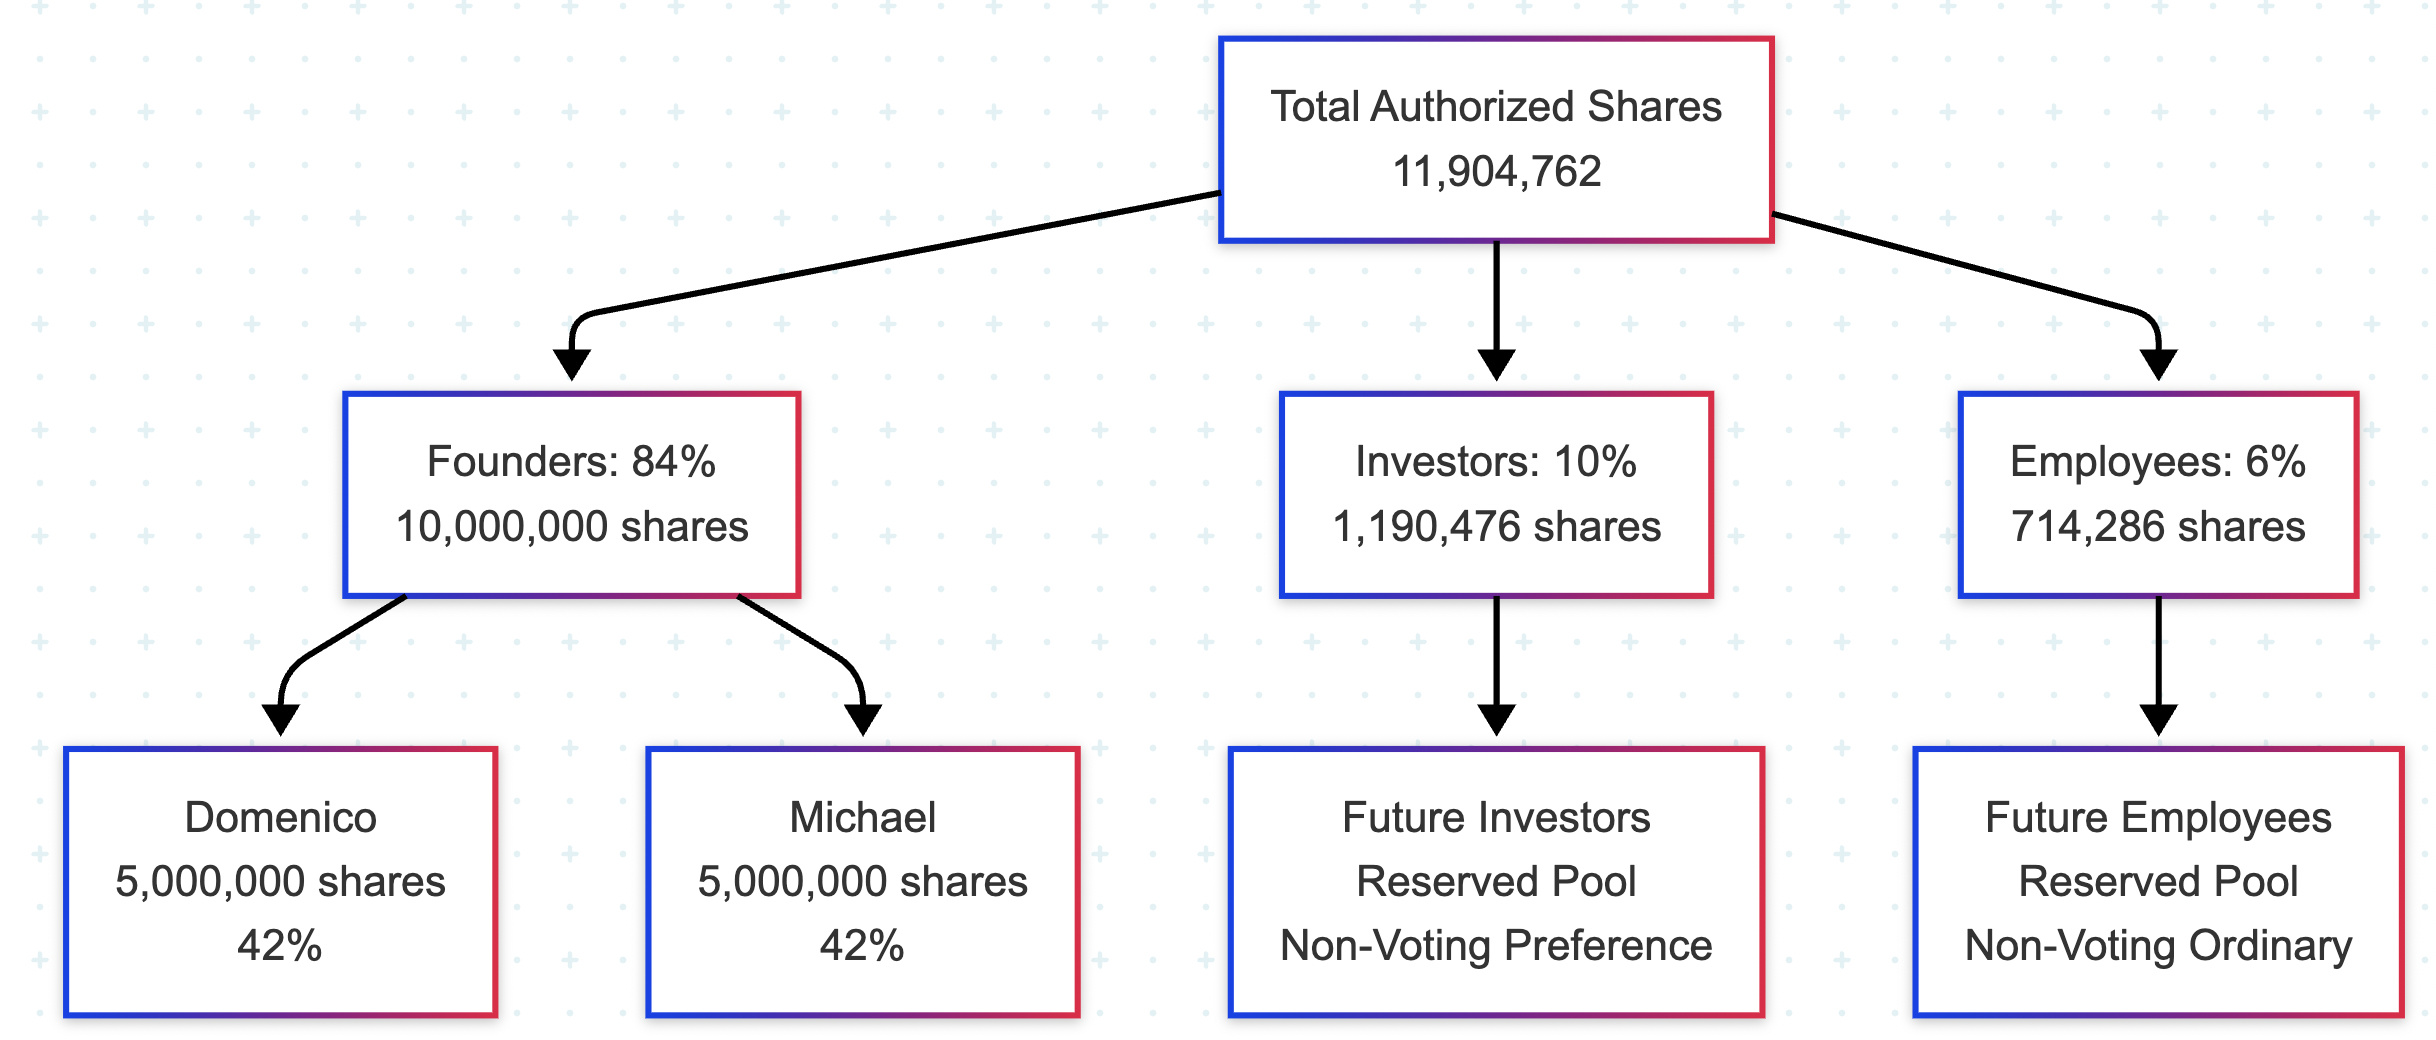
\includegraphics[width=0.9\textwidth]{/Users/domrutili/PROJECTS/Augmented-4-ShareHolder-Agreement/images/shares.png}
\end{center}

\textbf{Diagram Description:} The above diagram illustrates the hierarchical distribution of The Augmented 4 Pty Ltd's authorized share capital. At the top level, the total authorized shares of 11,904,762 are divided into three main categories: Founders (84\% - 10,000,000 shares), Investors (10\% - 1,190,476 shares), and Employees (6\% - 714,286 shares). The Founders category is further subdivided equally between Domenico and Michael, each holding 5,000,000 shares representing 42\% of the total. The Investor and Employee categories represent reserved pools for future allocation, with investors receiving Non-Voting Preference shares and employees receiving Non-Voting Ordinary shares. This visual representation demonstrates the balanced approach to equity distribution while maintaining founder control through voting rights concentration.

\textit{Note: This structure ensures founder control while providing appropriate investor protections and employee economic participation. All share issuances from reserved pools require unanimous Board approval and compliance with this Agreement.} 
\clearpage

% Schedule 2
% Content for sections/Schedule_2_Reserved_Matters.tex
\section*{SCHEDULE 2 - RESERVED MATTERS}

The following matters require approval as specified below:

\subsection*{Part A: Matters Requiring Unanimous Shareholder Approval}
\textit{(Unanimous approval of all Shareholders required)}

\begin{enumerate}[label=\arabic*.]
    \item \textbf{Share Capital and Equity Structure:}
        \begin{enumerate}[label=(\alph*)]
            \item Issuance of any new shares or securities convertible into shares;
            \item Creation, amendment, or termination of any share class or rights;
            \item Any variation or abrogation of rights attaching to any shares;
            \item Any share buyback, capital reduction, or return of capital;
            \item Granting of options, warrants, or other equity instruments;
            \item Any transaction affecting the Reserved Share Pools.
        \end{enumerate}

    \item \textbf{Corporate Structure and Governance:}
        \begin{enumerate}[label=(\alph*)]
            \item Amendment of the Company's Constitution;
            \item Change of Company name or registered office;
            \item Appointment or removal of Directors;
            \item Determination of Director remuneration;
            \item Changes to Board composition or voting procedures;
            \item Adoption of any shareholder agreement amendments.
        \end{enumerate}

    \item \textbf{Major Business Decisions:}
        \begin{enumerate}[label=(\alph*)]
            \item Approval of annual business plans and budgets;
            \item Any expenditure exceeding AUD 1,000 (whether within or outside approved budget);
            \item Entry into expense contracts (excluding customer revenue contracts) with total value exceeding AUD 1,000 or duration longer than 12 months;
            \item Acquisition or disposal of assets exceeding AUD 50,000;
            \item Establishment of subsidiaries or joint ventures;
            \item Material changes to business strategy or operations.
        \end{enumerate}

    \item \textbf{Financial and Legal Matters:}
        \begin{enumerate}[label=(\alph*)]
            \item Borrowing exceeding AUD 100,000 or granting security;
            \item Declaration or payment of dividends;
            \item Appointment or removal of auditors;
            \item Commencement or settlement of material litigation;
            \item Any insolvency or winding up proceedings;
            \item Material tax elections or changes to accounting policies.
        \end{enumerate}

    \item \textbf{Intellectual Property and Technology:}
        \begin{enumerate}[label=(\alph*)]
            \item Assignment, licensing, or disposal of material IP rights;
            \item Filing, abandonment, or enforcement of patents or trademarks;
            \item Material technology development or R\&D decisions;
            \item Material AI model development or deployment decisions;
            \item Engagement of key technology consultants or advisors;
            \item Open source licensing or technology sharing arrangements;
            \item Data protection and privacy policy changes.
        \end{enumerate}
\end{enumerate}

\subsection*{Part B: Matters Requiring Ordinary Shareholder (Voting) Approval}
\textit{(Approval of holders of Ordinary Shares (Voting) required)}

\begin{enumerate}[label=\arabic*.]
    \item \textbf{Operational Decisions:}
        \begin{enumerate}[label=(\alph*)]
            \item Hiring or termination of senior executives;
            \item Employee compensation and benefit policies;
            \item Office lease agreements and relocations;
            \item Marketing and sales strategy decisions;
            \item Customer contract negotiations exceeding AUD 50,000;
            \item Supplier and vendor selection for material services.
        \end{enumerate}

    \item \textbf{Financial Management:}
        \begin{enumerate}[label=(\alph*)]
            \item Monthly and quarterly financial reporting;
            \item Banking arrangements and account management;
            \item Insurance coverage and risk management;
            \item Investment of surplus funds;
            \item Credit facilities and payment terms;
            \item Financial controls and approval authorities.
        \end{enumerate}

    \item \textbf{Emergency and Administrative Matters:}
        \begin{enumerate}[label=(\alph*)]
            \item Approval of expense policies and delegation of authorities;
            \item Review and ratification of emergency expenditures exceeding single Director limits;
            \item Establishment of petty cash and operational spending limits (up to AUD 1,000);
            \item Administrative approvals for routine operational matters under AUD 1,000.
        \end{enumerate}
\end{enumerate}

\subsection*{Part C: Information and Reporting Requirements}

\begin{enumerate}[label=\arabic*.]
    \item \textbf{Regular Reporting:}
        \begin{enumerate}[label=(\alph*)]
            \item Monthly management accounts within 15 business days;
            \item Quarterly financial and operational performance reviews;
            \item Annual audited financial statements;
            \item Technology development progress reports;
            \item Customer acquisition and retention metrics;
            \item Competitive analysis and market updates.
        \end{enumerate}

    \item \textbf{Strategic Updates:}
        \begin{enumerate}[label=(\alph*)]
            \item Business plan updates and revisions;
            \item Technology roadmap and development priorities;
            \item Market expansion and growth opportunities;
            \item Partnership and collaboration discussions;
            \item Regulatory and compliance developments;
            \item Risk assessment and mitigation strategies.
        \end{enumerate}
\end{enumerate}

\subsection*{Part D: Current Structure Notes}

\begin{enumerate}[label=\arabic*.]
    \item Current structure: 42/42/10/6 shareholding structure with founders holding equal voting control
    \item Founders maintain 100\% voting control through Ordinary Shares (Voting)
    \item Reserved pools provide for future investor and employee participation
    \item All Reserved Matters require unanimous founder approval given equal voting structure
    \item Preference Shareholders receive information rights and economic protections
    \item Employee Shareholders participate economically without governance rights
\end{enumerate}

\subsection*{Part E: Approval Thresholds Summary}

\begin{tabularx}{\textwidth}{@{} l X l @{}}
\textbf{Matter Type} & \textbf{Approval Required} & \textbf{Decision Makers} \\
\hline
Part A Matters & Unanimous Shareholders & Both Founders \\
Part B Matters & Ordinary Shareholders & Both Founders (effectively) \\
Future Investor Matters & As specified in investment terms & Per future agreements \\
Future Employee Matters & Unanimous Board approval & Both Founder-Directors \\
Board Decisions & Unanimous Board & Both Founder-Directors \\
Routine Operations & Management discretion & Within approved policies \\
\hline
\end{tabularx}

\vspace{1em}

\textbf{Notes:}
\begin{itemize}
    \item Current structure: 42/42/10/6 shareholding structure with founders holding equal voting control
    \item Founders maintain 100\% voting control through Ordinary Shares (Voting)
    \item Reserved pools provide for future investor and employee participation
    \item All Reserved Matters require unanimous founder approval given equal voting structure
    \item Preference Shareholders receive information rights and economic protections
    \item Employee Shareholders participate economically without governance rights
    \item This schedule will be updated when new share classes are implemented
\end{itemize} 
\clearpage

% Schedule 3
\section*{ANNEXURE A - FORM OF DEED OF ACCESSION}

\textbf{DEED OF ACCESSION}

\textbf{Date:} [Insert Date]

\textbf{Parties:}
\begin{enumerate}
    \item \textbf{[INSERT NAME OF NEW SHAREHOLDER]} of [Insert Address of New Shareholder] (the ``Acceding Shareholder'')
    \item \textbf{THE AUGMENTED 4 PTY LTD} (ACN 686 749 575) of Unit 4, 5 Norman Avenue, Dolls Point, New South Wales 2219, Australia (the ``Company'')
\end{enumerate}

\textbf{Recitals:}
\begin{enumerate}[label=\Alph*.]
    \item This Deed is supplemental to a Shareholders Agreement dated [9 June 2025] (the ``Shareholders Agreement'') made between (1) The Company, (2) Domenico Rutigliano, and (3) Michael Scheelhardt (collectively the ``Original Parties''), relating to the governance and affairs of the Company. A copy of the Shareholders Agreement has been provided to the Acceding Shareholder.
    \item The Acceding Shareholder has acquired or is about to acquire [Number] [Class, e.g., Ordinary] Shares in the Company (the ``Transferred Shares'') from [Name of Transferor Shareholder or ``the Company'' if new issue] (the ``Transferor'') and is required as a condition of such acquisition and registration of the Transferred Shares to execute this Deed.
    \item Capitalised terms used in this Deed have the meanings given to them in the Shareholders Agreement unless otherwise defined herein.
\end{enumerate}

\textbf{Operative Provisions:}
\begin{enumerate}
    \item \textbf{Accession to Shareholders Agreement}
    \begin{enumerate}[label=(\alph*)]
        \item The Acceding Shareholder hereby unconditionally and irrevocably covenants with the Company (for itself and as agent and trustee for each of the other parties to the Shareholders Agreement from time to time) that with effect from the date of this Deed (or, if later, the date of registration of the Transferred Shares in the name of the Acceding Shareholder), it will:
        \begin{enumerate}[label=(\roman*)]
            \item be bound by all the terms and provisions of the Shareholders Agreement in all respects as if the Acceding Shareholder were an original party to the Shareholders Agreement and named therein as a Shareholder; and
            \item observe, perform and be bound by all the covenants, obligations, and undertakings contained in the Shareholders Agreement that are applicable to a Shareholder (and specifically, if applicable, to the party from whom the Shares are being acquired or in whose place the Acceding Shareholder stands).
        \end{enumerate}
        \item The Acceding Shareholder confirms that it has been provided with a complete copy of the Shareholders Agreement (including all schedules and any amendments thereto) and has had the opportunity to take independent legal advice thereon.
    \end{enumerate}

    \item \textbf{Notices}
    \begin{enumerate}[label=(\alph*)]
        \item For the purposes of the notice provisions in the Shareholders Agreement, the Acceding Shareholder's address for notices is:
        \begin{itemize}
            \item Address: [Insert Acceding Shareholder's Full Address]
            \item Email: [Insert Acceding Shareholder's Email Address]
            \item Attn: [If applicable, e.g., Company Secretary if Acceding Shareholder is a company]
        \end{itemize}
    \end{enumerate}

    \item \textbf{Governing Law and Jurisdiction}
    \begin{enumerate}[label=(\alph*)]
        \item This Deed shall be governed by and construed in accordance with the laws of New South Wales, Australia.
        \item The parties submit to the exclusive jurisdiction of the courts of New South Wales, Australia in respect of all matters arising out of or in connection with this Deed.
    \end{enumerate}

    \item \textbf{Counterparts}
    \begin{enumerate}[label=(\alph*)]
        \item This Deed may be executed in any number of counterparts. All counterparts taken together will be taken to constitute one instrument.
    \end{enumerate}
\end{enumerate}

\vspace{1em}
\hrule
\vspace{1em}

\textbf{EXECUTION PAGE}

\textbf{Executed as a Deed.}

\vspace{2em}

\textbf{For the Acceding Shareholder:}

\begin{center}
\textit{(Execution block will vary depending on whether the Acceding Shareholder is an individual or a company)}
\end{center}

\vspace{1em}

\textbf{If an individual:}

\begin{tabular}{p{8cm}p{8cm}}
Signed, sealed and delivered by & In the presence of: \\
\textbf{[INSERT NAME OF ACCEDING} & \\
\textbf{SHAREHOLDER]} & \\
& \\
\cline{1-1}\cline{2-2} \\
\textit{Signature of Acceding Shareholder} & \textit{Signature of Witness} \\
& \\
& \cline{2-2} \\
& \textit{Name of Witness (print)} \\
& \\
& \cline{2-2} \\
& \textit{Address of Witness} \\
& \\
& \cline{2-2} \\
& \textit{Occupation of Witness} \\
\end{tabular}

\vspace{3em}

\textbf{If a company executing under s127 of the Corporations Act:}

\begin{tabular}{p{16cm}}
Executed by \textbf{[INSERT COMPANY NAME OF ACCEDING SHAREHOLDER]} \\
(ACN/ABN [Insert ACN/ABN]) in accordance with section 127(1) of the Corporations Act 2001 (Cth) by: \\
\\
\end{tabular}

\begin{tabular}{p{8cm}p{8cm}}
\cline{1-1}\cline{2-2} \\
\textit{Signature of Director} & \textit{Signature of Director/Company Secretary} \\
& \\
\cline{1-1}\cline{2-2} \\
\textit{Name of Director (print)} & \textit{Name of Director/Company Secretary (print)} \\
\end{tabular}

\vspace{3em}

\textbf{For the Company:}

\begin{tabular}{p{16cm}}
Executed by \textbf{THE AUGMENTED 4 PTY LTD} \\
(ACN 686 749 575) in accordance with section 127(1) of the Corporations Act 2001 (Cth) by: \\
\\
\end{tabular}

\begin{tabular}{p{8cm}p{8cm}}
\cline{1-1}\cline{2-2} \\
\textit{Signature of Director} & \textit{Signature of Director/Company Secretary} \\
& \\
\cline{1-1}\cline{2-2} \\
\textit{Name of Director (print)} & \textit{Name of Director/Company Secretary (print)} \\
\end{tabular} 
\clearpage

% Schedule 4
\section*{SCHEDULE 4 - COMPENSATION AND PROFIT SHARING STRUCTURE}

This Schedule outlines the compensation and profit sharing structure for The Augmented 4 Pty Ltd, establishing both salary provisions based on KPI achievement and profit distribution mechanisms aligned with the company's shareholding structure.

\section*{1. General Provisions}
\begin{enumerate}[label=\arabic*.]
\item \textbf{Effective Period:} This compensation and profit sharing structure commences from the Effective Date of this Agreement and continues for the duration of this Agreement.

\item \textbf{KPI Document Reference:} The specific Key Performance Indicators (KPIs) required for salary eligibility are detailed in a separate KPI Performance Document, which forms part of the operational framework of the Company but is maintained separately from this Agreement. The KPI Document may be updated from time to time by unanimous Board resolution to reflect changing business conditions and growth targets.

\item \textbf{Definition of Distributable Profit:} ``Distributable Profit'' means the net profit of the Company after:
    \begin{enumerate}[label=(\alph*)]
    \item All operating expenses and costs of goods sold;
    \item Founder salary payments (when KPI requirements are met);
    \item Tax obligations and statutory reserves;
    \item Mandatory working capital requirements;
    \item Research and development allocations as determined by the Board;
    \item Capital expenditure requirements as approved by the Board.
    \end{enumerate}

\item \textbf{Calculation Period:} Distributable Profit shall be calculated on a trimester basis (4-month periods): January-April, May-August, September-December.

\item \textbf{Board Certification:} The calculation of Distributable Profit must be certified by formal resolution of the Board of Directors, with both Directors required to sign off on the calculations.
\end{enumerate}

\section*{2. Founder Salary Structure}

\subsection*{2.1 KPI-Based Salary Eligibility}
\begin{enumerate}[label=\arabic*.]
\item \textbf{Salary Amounts:}
    \begin{enumerate}[label=(\alph*)]
    \item Domenico Rutigliano (CTO): AUD \$70,000 per annum
    \item Michael Scheelhardt (CRO): AUD \$70,000 per annum
    \end{enumerate}

\item \textbf{KPI Achievement Requirement:}
    \begin{enumerate}[label=(\alph*)]
    \item Salary payments are conditional upon achievement of KPIs as specified in the separate KPI Performance Document
    \item KPI achievement is measured and verified quarterly by the Board
    \item Both founders must contribute to overall KPI achievement for individual salary eligibility
    \item Partial KPI achievement may result in pro-rated salary payments at Board discretion
    \end{enumerate}

\item \textbf{Payment Terms:}
    \begin{enumerate}[label=(\alph*)]
    \item Salaries paid monthly in arrears, subject to KPI verification
    \item First salary payments commence upon first KPI achievement verification
    \item Salary payments take priority over profit distributions
    \item All salary payments subject to applicable tax withholdings and statutory deductions
    \end{enumerate}
\end{enumerate}

\subsection*{2.2 Business Operations Funding}
\begin{enumerate}[label=\arabic*.]
\item \textbf{Operational Reserve:} The Company shall maintain adequate funding for business operations, estimated at approximately AUD \$60,000 annually, which takes priority over both salary and profit distributions.

\item \textbf{Cash Flow Management:} Salary payments and operational funding requirements must be satisfied before any profit distributions are made to shareholders.

\item \textbf{Budget Review and Adjustment:} The Board may, by unanimous resolution, review and adjust the following budget allocations to reflect changing business conditions, market circumstances, or strategic requirements:
    \begin{enumerate}[label=(\alph*)]
    \item Founder salary amounts (currently AUD \$70,000 each per annum)
    \item Business operations funding (currently AUD \$60,000 per annum)
    \item Total compensation budget and allocation priorities
    \item Payment schedules and timing requirements
    \end{enumerate}

\item \textbf{Adjustment Process:} Any budget adjustments must be:
    \begin{enumerate}[label=(\alph*)]
    \item Documented in a formal Board resolution signed by both Directors
    \item Based on objective financial analysis and business justification
    \item Consistent with the Company's cash flow capacity and growth objectives
    \item Effective from a specified future date (not retrospectively applied)
    \item Communicated to all shareholders within 15 days of resolution
    \end{enumerate}
\end{enumerate}

\section*{3. Profit Distribution Structure}

\subsection*{3.1 Distribution Allocation}
\begin{enumerate}[label=\arabic*.]
\item \textbf{Founder Allocation:}
    \begin{enumerate}[label=(\alph*)]
    \item Domenico Rutigliano: 42\% of Distributable Profit
    \item Michael Scheelhardt: 42\% of Distributable Profit
    \end{enumerate}

\item \textbf{Investor Allocation:}
    \begin{enumerate}[label=(\alph*)]
    \item Future Investors: 10\% of Distributable Profit
    \item Held in reserve until investor shares are issued
    \item Upon investor share issuance, distributed proportionally among investors
    \end{enumerate}

\item \textbf{Employee Allocation:}
    \begin{enumerate}[label=(\alph*)]
    \item Employees and Advisors: 6\% of Distributable Profit
    \item Distributed through employee profit sharing program
    \item Allocation determined by Board based on performance and contribution
    \end{enumerate}
\end{enumerate}

\subsection*{3.2 Reserve Funds Management}
\begin{enumerate}[label=\arabic*.]
\item \textbf{Investor Reserve Fund:}
    \begin{enumerate}[label=(\alph*)]
    \item 10\% allocation held in designated reserve account
    \item Accumulates until investor shares are issued
    \item Upon investment, distributed to investors based on their shareholding
    \item If no investors after 3 years, Board may reallocate by unanimous resolution
    \end{enumerate}

\item \textbf{Employee Reserve Fund:}
    \begin{enumerate}[label=(\alph*)]
    \item 6\% allocation held in designated employee profit sharing account
    \item Distributed annually based on Board-approved criteria
    \item Includes performance bonuses, retention incentives, and recognition awards
    \item Unused amounts carry forward to subsequent years
    \end{enumerate}
\end{enumerate}

\section*{4. Payment Terms and Conditions}

\subsection*{4.1 Payment Schedule}
\begin{enumerate}[label=\arabic*.]
\item \textbf{Trimester Payments:}
    \begin{enumerate}[label=(\alph*)]
    \item Profit calculations completed within 30 days of trimester end
    \item Founder payments made within 60 days of trimester end
    \item Employee distributions made within 90 days of trimester end
    \item All payments subject to maintaining minimum cash reserves
    \end{enumerate}

\item \textbf{Minimum Cash Reserve Requirements:}
    \begin{enumerate}[label=(\alph*)]
    \item Company must maintain minimum \$100,000 cash reserves
    \item Additional reserves as determined by Board for operational needs
    \item Profit distributions suspended if reserves fall below minimum
    \end{enumerate}
\end{enumerate}

\subsection*{4.2 Financial Safeguards}
\begin{enumerate}[label=\arabic*.]
\item \textbf{Business Continuity Protection:}
    \begin{enumerate}[label=(\alph*)]
    \item Profit distributions must not impair business operations
    \item R\&D funding requirements take priority over distributions
    \item Growth opportunities funding protected
    \item Working capital needs fully satisfied before distributions
    \end{enumerate}

\item \textbf{Maximum Distribution Limits:}
    \begin{enumerate}[label=(\alph*)]
    \item Individual founder distributions capped at \$500,000 per calendar year
    \item Excess amounts carried forward to following year
    \item Board may increase caps by unanimous resolution
    \item Emergency business needs override distribution caps
    \end{enumerate}
\end{enumerate}

\section*{5. Documentation and Verification}

\subsection*{5.1 Financial Reporting}
\begin{enumerate}[label=\arabic*.]
\item \textbf{Quarterly Financial Statements:}
    \begin{enumerate}[label=(\alph*)]
    \item Profit and loss statements prepared by qualified accountant
    \item Balance sheet showing cash reserves and working capital
    \item Cash flow statements demonstrating business sustainability
    \item Detailed breakdown of profit calculations and allocations
    \end{enumerate}

\item \textbf{Transparency Requirements:}
    \begin{enumerate}[label=(\alph*)]
    \item Monthly financial summaries provided to all parties
    \item Quarterly detailed profit sharing reports
    \item Annual review of allocation percentages and criteria
    \item Access to relevant financial records for verification
    \end{enumerate}
\end{enumerate}

\subsection*{5.2 Approval Process}
\begin{enumerate}[label=\arabic*.]
\item \textbf{Board Approval Requirements:}
    \begin{enumerate}[label=(\alph*)]
    \item Unanimous Board resolution for profit calculations
    \item Both founders must approve distribution amounts
    \item Documented rationale for any distribution adjustments
    \item Quarterly review of financial performance and projections
    \end{enumerate}

\item \textbf{Dispute Resolution:}
    \begin{enumerate}[label=(\alph*)]
    \item Independent accountant review for calculation disputes
    \item Mediation process for allocation disagreements
    \item Final determination by Board unanimous resolution
    \item External audit rights for verification
    \end{enumerate}
\end{enumerate}

\section*{6. Additional Terms}

\begin{enumerate}[label=\arabic*.]
\item \textbf{Tax Treatment:}
    \begin{enumerate}[label=(\alph*)]
    \item Founder distributions treated as performance bonuses
    \item Employee distributions subject to payroll tax requirements
    \item All distributions subject to applicable statutory deductions
    \item Tax advice recommended for optimal structuring
    \end{enumerate}

\item \textbf{Adjustment Mechanisms:}
    \begin{enumerate}[label=(\alph*)]
    \item Allocation percentages may be reviewed annually
    \item Market conditions may trigger structure review
    \item Business model changes may require adjustments
    \item Force majeure events considered for temporary modifications
    \end{enumerate}

\item \textbf{Integration with Shareholding:}
    \begin{enumerate}[label=(\alph*)]
    \item Profit sharing percentages align with shareholding structure
    \item Changes to share structure may trigger profit sharing adjustments
    \item New shareholders automatically included in profit sharing
    \item Exit events override profit sharing arrangements
    \end{enumerate}

\item \textbf{Performance Incentives:}
    \begin{enumerate}[label=(\alph*)]
    \item Employee profit sharing based on performance metrics
    \item Board discretion for exceptional contribution bonuses
    \item Annual performance reviews determine individual allocations
    \item Long-term incentive alignment with company growth
    \end{enumerate}
\end{enumerate}

\textit{Note: This Schedule establishes a comprehensive compensation structure combining KPI-based salaries with profit sharing mechanisms that align with the company's shareholding structure. The structure ensures founders receive regular compensation when performance targets are met, while all stakeholders benefit proportionally from the company's success through profit distributions. The Board may, by unanimous resolution, adjust this structure if business conditions or strategic direction materially changes, provided such changes are documented and signed by all parties to this Agreement.} 
\clearpage

% Schedule 5
\section*{SCHEDULE 5 - PRE-EXISTING INTELLECTUAL PROPERTY CONTRIBUTIONS}

This Schedule sets out the pre-existing intellectual property rights (``Pre-existing IP'') owned by the Shareholders prior to the incorporation of the Company and contributed to the Company pursuant to the Intellectual Property and Confidentiality section of this Agreement.

\section*{1. Pre-existing IP Contributed by Domenico Rutigliano}

The following Pre-existing IP is owned by Domenico Rutigliano and is licensed to the Company under an exclusive, worldwide, royalty-free license until receipt of the full AUD 100,000 payment as specified in the Intellectual Property and Confidentiality section of this Agreement. Upon receipt of such payment, this Pre-existing IP shall be irrevocably assigned to the Company in full:

\standardtable{
Voice Agent Technology & Core AI voice agent architecture and algorithms & Developed between January 2023 and April 2025, including all source code, design documents, and technical specifications \\
\hline
Machine Learning Models & Trained AI models for voice recognition and natural language processing & Includes trained model weights, training methodologies, and performance metrics \\
\hline
Voice Synthesis Engine & Text-to-speech module with natural-sounding voices & Voice synthesis technology with customizable voice profiles \\
\hline
Voice Recognition System & Speech-to-text system with high accuracy & Includes noise cancellation algorithms and speaker recognition capabilities \\
\hline
Training Datasets & Curated voice datasets used for AI training & Anonymized voice recordings with associated transcriptions and metadata \\
\hline
Domain Names & Domain name registrations and associated digital assets & All rights to domain name augmentium.ai, including registration rights, renewal rights, and all associated account credentials. Also includes the email address theaugmented4.ai@gmail.com which serves as the management account for these digital assets. \\
\hline
Technical Documentation & Design documentation, architectural plans, and technical specifications & All documents describing the technology, implementation, and operation \\
\hline
Brand Assets & Preliminary logo designs, brand concepts, and company name & All design files and conceptual materials \\
}

\section*{2. Pre-existing IP Contributed by Michael Scheelhardt}

The following Pre-existing IP is owned by Michael Scheelhardt and is hereby irrevocably assigned to the Company in full with effect from the Effective Date:

\standardtable{
Market Research & Comprehensive analysis of AI voice agent market & Market sizing, competitor analysis, and opportunity assessment documentation \\
\hline
Business Model & Business model designs and revenue projections & Financial models, pricing strategies, and market entry plans \\
\hline
Customer Journey Maps & End-to-end customer experience mapping & User flow diagrams and experience design documents \\
\hline
Sales Materials & Initial sales pitch decks and marketing materials & Presentation materials, brochures, and digital assets \\
\hline
Go-to-Market Strategy & Detailed plans for product launch and scaling & Strategy documents, timelines, and implementation roadmaps \\
\hline
Pre-Existing Customer Relationships & Pre-existing industry contacts, customer relationships, and professional network existing prior to joining the Company & \textbf{Clarification:} This refers only to Michael's personal contacts and relationships established before the Effective Date. These remain Michael's personal property and are not assigned to the Company, although Michael grants the Company a non-exclusive right to leverage these relationships for business development. For avoidance of doubt, any new customer relationships, contacts, or business connections developed after the Effective Date while performing duties for the Company shall belong exclusively to the Company. \\
\hline
Domain Names & Domain name registrations and associated digital assets & All rights to domain names ta4.ai and augmented4.ai, including registration rights, renewal rights, and all associated account credentials. \\
}

\section*{3. Assignment Confirmation}

By signing this Agreement, each of Domenico Rutigliano and Michael Scheelhardt hereby:

\begin{enumerate}[label=(\alph*)]
\item confirms that they own all rights, title, and interest in and to their respective Pre-existing IP listed above and have full right, power, and authority to assign these rights to the Company;
\item irrevocably assigns to the Company all of their right, title, and interest in and to their respective Pre-existing IP, including all intellectual property rights therein, with effect from the Effective Date;
\item agrees to execute any further documents and to do all such other things as may be required to perfect the Company's title to the Pre-existing IP and to assist with its registration (where applicable) and protection; and
\item to the extent permitted by law, waives all moral rights and similar rights in respect of the Pre-existing IP.
\end{enumerate}

\section*{4. Third-Party IP}

The Shareholders acknowledge that the Pre-existing IP described above does not infringe the intellectual property rights of any third party. If any component of the Pre-existing IP incorporates third-party intellectual property rights, the relevant Shareholder shall ensure that appropriate licenses are obtained for the Company's use and exploitation of such third-party intellectual property rights, at no additional cost to the Company.

\section*{5. Future Updates}

This Schedule may be updated from time to time by written agreement of all Shareholders to include additional Pre-existing IP contributed to the Company after the Effective Date. 
\clearpage

% Schedule 6
\section*{SCHEDULE 6 - PERSONAL LOAN REGISTER}

This Schedule documents personal loans provided by Michael Scheelhardt to Domenico Rutigliano that are subject to repayment obligations under the Intellectual Property and Confidentiality section of this Agreement.

\section*{1. Loan Documentation Framework}

\begin{enumerate}[label=\arabic*.]
\item \textbf{Legal Status:} The personal loans documented in this Schedule are separate contractual obligations independent of this Shareholders Agreement, but are incorporated by reference for repayment enforcement purposes.

\item \textbf{Loan Register Maintenance:} This Schedule shall be updated by written agreement of both Michael Scheelhardt and Domenico Rutigliano to reflect:
    \begin{enumerate}[label=(\alph*)]
    \item New loans advanced
    \item Partial repayments made
    \item Interest adjustments (if any)
    \item Final loan balances
    \end{enumerate}

\item \textbf{Documentation Requirements:} Each loan entry must include:
    \begin{enumerate}[label=(\alph*)]
    \item Date of loan advance
    \item Principal amount
    \item Purpose of loan
    \item Repayment terms (if different from this Agreement)
    \item Outstanding balance as at the Effective Date
    \end{enumerate}
\end{enumerate}

\section*{2. Current Loan Register}

\textit{Note: The following table should be completed with actual loan details. This template provides the structure for documenting all personal loans.}

\begin{tabularx}{\textwidth}{@{} l l l X l @{}}
\textbf{Loan Date} & \textbf{Principal} & \textbf{Purpose} & \textbf{Description} & \textbf{Outstanding Balance} \\
\hline
[Date] & AUD [Amount] & [Purpose] & [Description of loan purpose and circumstances] & AUD [Balance] \\
\hline
[Date] & AUD [Amount] & [Purpose] & [Description of loan purpose and circumstances] & AUD [Balance] \\
\hline
[Date] & AUD [Amount] & [Purpose] & [Description of loan purpose and circumstances] & AUD [Balance] \\
\hline
\textbf{TOTAL} & & & & \textbf{AUD [Total Outstanding]} \\
\end{tabularx}

\section*{3. Loan Terms and Conditions}

\begin{enumerate}[label=\arabic*.]
\item \textbf{Interest Rate:} All personal loans are interest-free unless otherwise specified in individual loan documentation.

\item \textbf{Repayment Terms:} 
    \begin{enumerate}[label=(\alph*)]
    \item \textbf{Primary Repayment:} Full repayment upon Domenico's receipt of AUD 100,000 IP compensation
    \item \textbf{Alternative Repayment:} Monthly installments proportional to revenue-sharing IP compensation if applicable
    \item \textbf{No Demand:} Loans are not repayable on demand except as specified in this Agreement
    \end{enumerate}

\item \textbf{Security:} Loans secured against Domenico Rutigliano Assets as defined in the personal loan agreement with Michael Scheelhardt.

\item \textbf{Default:} Material breach of this Shareholders Agreement constitutes default under the personal loans.
\end{enumerate}

\section*{4. Acknowledgments and Confirmations}

\begin{enumerate}[label=\arabic*.]
\item \textbf{Michael Scheelhardt Confirms:}
    \begin{enumerate}[label=(\alph*)]
    \item All loans listed were advanced from personal funds
    \item Loans were made in good faith to support business development
    \item No interest has been charged or is owing
    \item Outstanding balances are accurate as at the Effective Date
    \end{enumerate}

\item \textbf{Domenico Rutigliano Acknowledges:}
    \begin{enumerate}[label=(\alph*)]
    \item Receipt of all loan amounts listed
    \item Personal obligation to repay outstanding balances
    \item Agreement to repayment terms as specified in this Agreement
    \item No disputes regarding loan amounts or terms
    \end{enumerate}

\item \textbf{Company Acknowledgment:}
    \begin{enumerate}[label=(\alph*)]
    \item The Company acknowledges these personal loan arrangements
    \item The Company is not a party to or guarantor of these loans
    \item Repayment obligations are incorporated for commercial certainty only
    \item These arrangements do not affect shareholding or governance rights
    \end{enumerate}
\end{enumerate}

\section*{5. Amendment and Updates}

\begin{enumerate}[label=\arabic*.]
\item \textbf{Loan Register Updates:} This Schedule may be updated by written agreement signed by both Michael Scheelhardt and Domenico Rutigliano.

\item \textbf{New Loans:} Additional personal loans may be added to this Schedule with:
    \begin{enumerate}[label=(\alph*)]
    \item Written documentation of loan terms
    \item Signatures of both parties
    \item Updated total outstanding balance
    \item Board notification within 30 days
    \end{enumerate}

\item \textbf{Repayment Recording:} Partial or full repayments shall be recorded with:
    \begin{enumerate}[label=(\alph*)]
    \item Date of repayment
    \item Amount repaid
    \item Updated outstanding balance
    \item Signatures confirming repayment
    \end{enumerate}
\end{enumerate}

\section*{6. Legal Framework}

\begin{enumerate}[label=\arabic*.]
\item \textbf{Governing Law:} Personal loans are governed by the laws of New South Wales, Australia.

\item \textbf{Dispute Resolution:} Disputes regarding personal loans are subject to the same dispute resolution mechanisms as this Shareholders Agreement.

\item \textbf{Enforceability:} This Schedule creates binding obligations enforceable independently of the Shareholders Agreement.

\item \textbf{Tax Implications:} Each party is responsible for their own tax obligations arising from these loan arrangements.
\end{enumerate}

\textit{Note: This Schedule should be completed with actual loan details before execution of this Agreement. The parties may also choose to execute separate formal loan agreements that are then summarized in this Schedule for reference purposes.} 
\clearpage

% Annexure A
\section*{ANNEXURE A - KEY PERFORMANCE INDICATORS DOCUMENT}

This Annexure sets out the specific Key Performance Indicators (KPIs) referenced in Schedule 4 of the Shareholders Agreement, establishing the performance targets required for founder salary eligibility.

\section*{1. KPI Achievement Period}

\begin{enumerate}[label=\arabic*.]
\item \textbf{Performance Period:} June 2025 to July 2025 (2-month achievement window)
\item \textbf{Measurement Date:} 31 July 2025
\item \textbf{Verification Process:} Board resolution required within 15 days of measurement date
\item \textbf{Salary Commencement:} August 2025 (upon successful KPI verification)
\end{enumerate}

\section*{2. Michael Scheelhardt (CRO) - Customer Acquisition KPIs}

\subsection*{2.1 Primary Target}
\begin{enumerate}[label=\arabic*.]
\item \textbf{Customer Acquisition Target:} Secure 50 enterprise customers by 31 July 2025
\item \textbf{Revenue Requirement:} Minimum AUD \$200,000 annual recurring revenue from acquired customers
\item \textbf{Customer Definition:} ``Enterprise Customer'' means a business entity with a signed service agreement generating minimum AUD \$4,000 annual revenue to the Company
\end{enumerate}

\subsection*{2.2 Acquisition Methods}
\begin{enumerate}[label=\arabic*.]
\item \textbf{Personal Engagement:}
    \begin{enumerate}[label=(\alph*)]
    \item Direct sales activities and customer meetings
    \item Relationship building and business development
    \item Contract negotiation and closing
    \item Customer onboarding coordination
    \end{enumerate}

\item \textbf{Sales Agent Recruitment:}
    \begin{enumerate}[label=(\alph*)]
    \item Identify, recruit, and sign sales agents
    \item Establish agent commission structures and agreements
    \item Provide sales training and support materials
    \item Monitor and manage agent performance
    \end{enumerate}

\item \textbf{Partnership Development:}
    \begin{enumerate}[label=(\alph*)]
    \item Establish strategic partnerships for customer referrals
    \item Negotiate partnership agreements and revenue sharing
    \item Develop joint marketing and sales initiatives
    \item Maintain ongoing partner relationships
    \end{enumerate}
\end{enumerate}

\subsection*{2.3 Success Metrics}
\begin{enumerate}[label=\arabic*.]
\item \textbf{Quantitative Targets:}
    \begin{enumerate}[label=(\alph*)]
    \item Minimum 50 signed enterprise customers
    \item Minimum AUD \$200,000 annual recurring revenue
    \item Average customer value of AUD \$4,000 per annum
    \item Customer contracts with minimum 12-month terms
    \end{enumerate}

\item \textbf{Quality Requirements:}
    \begin{enumerate}[label=(\alph*)]
    \item Customers must be creditworthy and financially viable
    \item Signed contracts must be legally binding and enforceable
    \item Payment terms must align with Company cash flow requirements
    \item Customer onboarding must be completed within 30 days of signing
    \end{enumerate}
\end{enumerate}

\section*{3. Domenico Rutigliano (CTO) - Technical Delivery KPIs}

\subsection*{3.1 Primary Target}
\begin{enumerate}[label=\arabic*.]
\item \textbf{Automated Onboarding System:} Deliver a complete automated customer onboarding system by 31 July 2025
\item \textbf{Automation Level:} Achieve 100\% automation for standard customer onboarding processes
\item \textbf{Scalability Requirement:} System must handle minimum 50 concurrent customer onboardings
\end{enumerate}

\subsection*{3.2 Technical Specifications}
\begin{enumerate}[label=\arabic*.]
\item \textbf{Automated Onboarding Features:}
    \begin{enumerate}[label=(\alph*)]
    \item Self-service customer registration portal
    \item Automated account setup and configuration
    \item Automated service provisioning and activation
    \item Automated welcome communications and documentation
    \item Automated billing setup and payment processing integration
    \end{enumerate}

\item \textbf{System Integration:}
    \begin{enumerate}[label=(\alph*)]
    \item Integration with existing customer management systems
    \item API connections for third-party service providers
    \item Automated data synchronization across platforms
    \item Real-time status tracking and reporting
    \end{enumerate}

\item \textbf{Quality Assurance:}
    \begin{enumerate}[label=(\alph*)]
    \item Comprehensive testing of all automated processes
    \item Error handling and exception management
    \item System monitoring and alerting capabilities
    \item Documentation and user guides
    \end{enumerate}
\end{enumerate}

\subsection*{3.3 Ongoing Customer Onboarding}
\begin{enumerate}[label=\arabic*.]
\item \textbf{Current Process Enhancement:}
    \begin{enumerate}[label=(\alph*)]
    \item Maintain and improve existing 80\% automated onboarding process
    \item Continue onboarding new customers acquired by Michael
    \item Ensure seamless transition from semi-automated to fully automated system
    \item Provide technical support for customer onboarding issues
    \end{enumerate}

\item \textbf{Performance Standards:}
    \begin{enumerate}[label=(\alph*)]
    \item Maximum 24-hour onboarding completion time for standard customers
    \item 99\% system uptime during onboarding processes
    \item Zero critical errors in automated onboarding workflows
    \item Customer satisfaction score of 4.5/5 or higher for onboarding experience
    \end{enumerate}
\end{enumerate}

\section*{4. Interdependent Success Factors}

\begin{enumerate}[label=\arabic*.]
\item \textbf{Collaborative Requirements:}
    \begin{enumerate}[label=(\alph*)]
    \item Michael's customer acquisition must align with Domenico's technical delivery timeline
    \item Domenico's automated system must support Michael's customer volume targets
    \item Both founders must coordinate to ensure smooth customer onboarding experience
    \item Regular progress meetings and status updates required throughout the performance period
    \end{enumerate}

\item \textbf{Mutual Support Obligations:}
    \begin{enumerate}[label=(\alph*)]
    \item Michael must provide customer requirements and feedback to inform technical development
    \item Domenico must provide technical specifications and limitations to guide sales efforts
    \item Both founders must participate in customer demonstrations and technical presentations as required
    \item Shared responsibility for customer satisfaction and retention
    \end{enumerate}
\end{enumerate}

\section*{5. KPI Verification and Assessment}

\subsection*{5.1 Documentation Requirements}
\begin{enumerate}[label=\arabic*.]
\item \textbf{Michael's Deliverables:}
    \begin{enumerate}[label=(\alph*)]
    \item Signed customer contracts with revenue details
    \item Sales agent agreements and partnership contracts
    \item Customer onboarding status reports
    \item Revenue projection and cash flow analysis
    \end{enumerate}

\item \textbf{Domenico's Deliverables:}
    \begin{enumerate}[label=(\alph*)]
    \item Completed automated onboarding system with full documentation
    \item System testing reports and quality assurance documentation
    \item Performance metrics and system monitoring reports
    \item User guides and technical documentation
    \end{enumerate}
\end{enumerate}

\subsection*{5.2 Board Assessment Process}
\begin{enumerate}[label=\arabic*.]
\item \textbf{Evaluation Criteria:}
    \begin{enumerate}[label=(\alph*)]
    \item Quantitative target achievement (50 customers, \$200K revenue, 100\% automation)
    \item Quality of deliverables and customer satisfaction
    \item Timeline adherence and milestone completion
    \item Collaborative effectiveness and mutual support
    \end{enumerate}

\item \textbf{Assessment Outcomes:}
    \begin{enumerate}[label=(\alph*)]
    \item \textbf{Full Success:} Both founders achieve all KPIs - full salary eligibility commences
    \item \textbf{Partial Success:} One founder achieves KPIs - pro-rated salary consideration at Board discretion
    \item \textbf{Collective Shortfall:} Neither founder fully achieves KPIs - salary eligibility deferred pending revised targets
    \item \textbf{Force Majeure:} External factors prevent achievement - Board may adjust targets or timeline
    \end{enumerate}
\end{enumerate}

\section*{6. Financial Impact and Cash Flow Model}

\begin{enumerate}[label=\arabic*.]
\item \textbf{Revenue Target Achievement:}
    \begin{enumerate}[label=(\alph*)]
    \item 50 enterprise customers × AUD \$4,000 = AUD \$200,000 annual revenue
    \item Monthly recurring revenue: AUD \$16,667
    \item Quarterly revenue: AUD \$50,000
    \end{enumerate}

\item \textbf{Cost Structure Upon Success:}
    \begin{enumerate}[label=(\alph*)]
    \item Domenico salary: AUD \$70,000 per annum (AUD \$5,833 monthly)
    \item Michael salary: AUD \$70,000 per annum (AUD \$5,833 monthly)
    \item Business operations: AUD \$60,000 per annum (AUD \$5,000 monthly)
    \item Total fixed costs: AUD \$200,000 per annum (AUD \$16,667 monthly)
    \end{enumerate}

\item \textbf{Break-Even Analysis:}
    \begin{enumerate}[label=(\alph*)]
    \item Revenue target exactly matches cost structure
    \item Additional customers beyond 50 generate profit for bonus distributions
    \item System scalability supports growth beyond initial targets
    \item Automated processes reduce marginal costs for additional customers
    \end{enumerate}
\end{enumerate}

\textit{Note: This KPI Document forms an integral part of the compensation structure outlined in Schedule 4 of the Shareholders Agreement. Achievement of these KPIs is essential for salary eligibility and represents the foundation for the Company's growth and financial sustainability. The Board may, by unanimous resolution, modify these KPIs if material changes in market conditions or business circumstances warrant adjustment, provided such modifications are documented and agreed to by all parties.} 

% Add any further schedules here using the same pattern  % This master file inputs Schedule_1, Schedule_2, Schedule_3, Schedule_4_KPIs

\end{document} 